\documentclass[12pt,a4paper]{report}
\usepackage{iftex}
% XeTeX/LuaTeX (tectonic): Unicode Latin Modern so Vietnamese diacritics render.
\ifTUTeX
  \usepackage{fontspec}
\else
  \usepackage[T1]{fontenc}
  \usepackage[utf8]{inputenc}
  \usepackage{lmodern}
\fi
\usepackage[english]{babel}
\usepackage[left=3cm,right=2.5cm,top=2.5cm,bottom=2.5cm]{geometry}
\usepackage{setspace}
\usepackage{graphicx}
\usepackage{booktabs}
\usepackage{array}
\usepackage{tabularx}
\usepackage{longtable}
\usepackage{amsmath,amssymb}
\usepackage{enumitem}
\usepackage{xcolor}
\usepackage{microtype}
\usepackage{caption}
\usepackage{subcaption}
\usepackage{float}
\usepackage[hidelinks]{hyperref}
\usepackage{xurl}
\usepackage[numbers,sort&compress]{natbib}
\usepackage{fancyhdr}
\usepackage{listings}
\usepackage{tikz}
\usetikzlibrary{positioning,fit,arrows.meta,calc}

\graphicspath{{figures/}{../results/danang_protocol_v1/summary/}}
\onehalfspacing
\setlength{\parindent}{1.25cm}
\setlength{\parskip}{0.15em}
\setlength{\emergencystretch}{2em}
\pagestyle{fancy}
\fancyhf{}
\fancyhead[R]{\thepage}
\fancyhead[L]{Evidence-Aware RL for Da Nang Signal Control}
\renewcommand{\headrulewidth}{0.3pt}
\captionsetup{font=small,labelfont=bf}
\hypersetup{pdftitle={Evidence-Aware Reinforcement Learning for Da Nang Traffic Signal Control: From an Empirical Intersection Anchor to a District-Scale Experiment},pdfauthor={Luong Quang Khang}}

\newcommand{\qint}{\ensuremath{Q_{\mathrm{int}}}}
\newcommand{\ddqn}{Dueling Double DQN}
% Name of the two-tier evaluation framework (not a new RL algorithm).
\newcommand{\methodname}{EA-TSC}

\begin{document}
\hypersetup{pageanchor=false}

\begin{titlepage}
\centering
{\large MINISTRY OF EDUCATION AND TRAINING\par}
{\large FPT UNIVERSITY\par}
\vspace{2.2cm}
{\Large\bfseries EVIDENCE-AWARE REINFORCEMENT LEARNING\\[0.25cm]
FOR DA NANG TRAFFIC SIGNAL CONTROL\\[0.25cm]
FROM AN EMPIRICAL INTERSECTION ANCHOR\\[0.25cm]
TO A DISTRICT-SCALE EXPERIMENT\par}
\vspace{1.8cm}
{\large A thesis submitted in partial fulfillment of the requirements\\
for the degree of Master of Software Engineering\par}
\vspace{1.5cm}
{\Large\bfseries Luong Quang Khang\par}
\vfill
\begin{tabular}{ll}
Supervisor: & Dr. Le Van Minh
\end{tabular}
\vfill
{\large Da Nang, Vietnam --- 2026\par}
\end{titlepage}

\pagenumbering{roman}
\hypersetup{pageanchor=true}
\chapter*{Declaration}
I declare that this thesis reports the experiment protocol and results contained in the accompanying repository. Published traffic observations and prior methods are attributed to their sources. The interpretations, implementation, experiment design, and analysis are the author's work. The repository retains machine-readable manifests, evaluation records, and calculation scripts. Some CityFlow checkpoints and raw replays remain local files excluded from Git; the evidence appendix records this reproducibility limit and preserves selected configuration and selection records.

\chapter*{Acknowledgements}
I thank my supervisor, Dr. Le Van Minh, for his guidance. I also acknowledge the authors who made the Da Nang intersection observations public and the developers of SUMO, CityFlow, and OpenStreetMap, whose open tools and data made this reproducible study possible.

\chapter*{Abstract}
This thesis studies adaptive traffic signal control in Da Nang, Vietnam, through two deliberately separated evidence tiers. The empirical anchor reconstructs the Le Thanh Nghi--Cach Mang Thang 8--2/9 intersection in SUMO from a published 103-second signal plan, an audited OpenStreetMap snapshot, a twelve-movement traffic table reported from 2022 data, and four hourly camera movement lines collected on 1 April 2025. The camera lines provide approximate, digitized published vehicle counts: 1,395 vehicles in the normal hour at 13:00, 2,330 in the morning peak at 08:00, and 2,400 in the evening peak at 17:00. The second tier implements a 53-signal OpenStreetMap-derived Hai Chau topology in CityFlow. Its routes, flows, and signal plans are synthetic; only the temporal demand shape is constrained by published Da Nang evidence. It tests executable network scale and comparative controller behavior within a synthetic protocol. We call this two-tier, evidence-audited evaluation framework \methodname{} (Evidence-Aware Traffic Signal Control); it is a protocol for evaluating controllers, not a new RL algorithm.

At the empirical anchor, a \ddqn{} controller is trained for thirty one-hour episodes with five independent training seeds. A base DQN architecture is retained as an ablation. Published fixed-time, raw Max-Pressure, and hysteretic Max-Pressure controllers provide non-learning baselines. Over 1,000 additional paired demand realizations per regime, the published plan has a lower queue integral than raw Max-Pressure in all 3,000 comparisons and than hysteretic Max-Pressure in 2,999 of 3,000. Checkpoint selection uses a separate validation demand realization; testing uses fifteen held-out cases across three traffic regimes. The primary metric is the integral of stopped vehicles inside the model plus vehicles waiting to enter it. Uncertainty for the learning controller is calculated over training seeds, not over crossed simulator runs.

The empirical-anchor result is regime dependent. Relative to the published fixed plan, \ddqn{} changes the queue integral by $+320.7\%$ in normal demand, $-1.0\%$ in the morning peak, and $-34.5\%$ in the evening peak. The 95\% bootstrap intervals for the absolute paired changes are $[7.60,56.14]$, $[-9.47,8.49]$, and $[-69.55,-35.34]$ vehicle-hours, respectively. These findings motivate a demand-gating hypothesis with fixed-time fallback at this modelled junction; they do not establish field safety or a city-wide benefit. The 53-signal experiment defines a frozen 30-case split and a five-seed confirmatory protocol. The current thesis reports a separate bounded analysis of the completed matched cases and labels it explicitly; a strict confirmatory release is withheld until its fail-closed verifier passes.

In that bounded 53-signal analysis, a fresh regime gate that retains tuned fixed-time in normal and morning-peak demand and enables the residual policy only in the evening peak reduced the pooled-case queue integral for all five learning seeds, by 1.03\%--5.62\% (mean 3.48\%). All five seeds have fresh fifteen-case coverage; seeds 13 and 16 use fresh fixed-time normal/AM replays and fresh residual PM replays. The gate was chosen after inspecting test behavior, and the original validation selector rejected seeds 13 and 16. This is exploratory evidence conditional on retained cases, not an independently confirmed benefit.

A separate feasibility demonstration applies a VisDrone-trained YOLO detector, ByteTrack tracking, and line counting to fifteen minutes of a public Da Nang traffic camera. It recovers car turning probabilities at two junctions and runs faster than real time for one camera, but it has no hand-count validation and supplies no input to either simulator.

\noindent\textbf{Keywords:} traffic signal control; reinforcement learning; Dueling Double DQN; SUMO; CityFlow; Da Nang; reproducibility; mixed traffic.

\tableofcontents
\listoffigures
\listoftables
\clearpage
\pagenumbering{arabic}

\chapter{Introduction}

\section{Motivation}
Traffic signal control is a sequential decision problem under uncertain demand. A fixed plan is predictable and inexpensive, but it cannot directly react when queues shift between approaches. Reinforcement learning (RL) offers a way to learn a feedback policy from repeated interaction with a traffic model. Its flexibility also introduces risks: a controller can exploit modelling artifacts, results can depend strongly on random seed, and an apparent improvement can disappear outside the trained demand regime.

Da Nang is a particularly relevant setting because traffic is heterogeneous and motorcycle dominated. Earlier local work has framed signal timing around surveyed arterial flows: a 2007 study designed coordinated green-wave timing for several Da Nang arterials from field flow surveys~\cite{tran2007greenwave}. The most useful public evidence found for this study is the detailed case study by Phan, Le, and Nguyen~\cite{phan2025danang}. It identifies the target signal, reports its geometry and 103-second timing plan, gives a twelve-movement table based on 2022 traffic-volume data, and publishes four camera movement profiles collected on 1 April 2025. That evidence can anchor one junction, but it cannot calibrate every signal in a district. The research design therefore keeps empirical fidelity and spatial scale as two distinct questions: a demand-matched isolated-junction study supports site-specific findings, while a synthetic 53-signal Hai Chau experiment tests whether the software, controller representation, and evaluation protocol scale.

Figure~\ref{fig:overview} summarizes the resulting framework, \methodname{}. Its two tiers share controllers, metrics, and an evidence audit, but they answer different questions and draw on different evidence.

\begin{figure}[H]
\centering
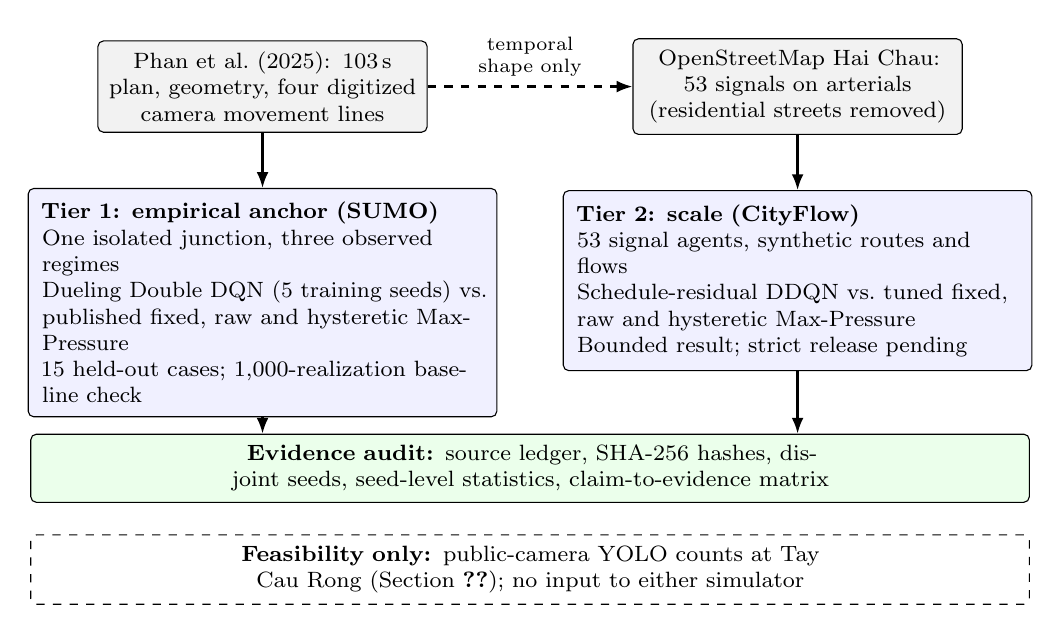
\begin{tikzpicture}[
  font=\footnotesize, node distance=4mm and 6mm,
  src/.style={draw, rounded corners=2pt, fill=gray!10, align=center, text width=3.9cm, inner sep=4pt},
  box/.style={draw, rounded corners=2pt, fill=blue!6, align=left, text width=5.6cm, inner sep=5pt},
  aud/.style={draw, rounded corners=2pt, fill=green!8, align=center, text width=12.4cm, inner sep=4pt},
  demo/.style={draw, dashed, rounded corners=2pt, align=center, text width=12.4cm, inner sep=4pt},
  arr/.style={-{Latex[length=2mm]}, thick}]
\node[src] (phan) {Phan et al.\ (2025): 103\,s plan, geometry, four digitized camera movement lines};
\node[src, right=2.6cm of phan] (osm) {OpenStreetMap Hai Chau: 53 signals on arterials (residential streets removed)};
\node[box, below=7mm of phan] (t1) {\textbf{Tier 1: empirical anchor (SUMO)}\\
One isolated junction, three observed regimes\\
\ddqn{} (5 training seeds) vs.\ published fixed, raw and hysteretic Max-Pressure\\
15 held-out cases; 1,000-realization baseline check};
\node[box, below=7mm of osm] (t2) {\textbf{Tier 2: scale (CityFlow)}\\
53 signal agents, synthetic routes and flows\\
Schedule-residual DDQN vs.\ tuned fixed, raw and hysteretic Max-Pressure\\
Bounded result; strict release pending};
\draw[arr] (phan) -- (t1);
\draw[arr] (osm) -- (t2);
\draw[arr, dashed] (phan.east) -- node[above, font=\scriptsize, align=center]{temporal\\shape only} (osm.west);
\node[aud, below=5mm of $(t1.south)!0.5!(t2.south)$] (audit) {\textbf{Evidence audit:} source ledger, SHA-256 hashes, disjoint seeds, seed-level statistics, claim-to-evidence matrix};
\draw[arr] (t1.south) -- (t1.south |- audit.north);
\draw[arr] (t2.south) -- (t2.south |- audit.north);
\node[demo, below=4mm of audit] {\textbf{Feasibility only:} public-camera YOLO counts at Tay Cau Rong (Section~\ref{sec:camera}); no input to either simulator};
\end{tikzpicture}
\caption{Overview of \methodname{}. Solid arrows show where evidence enters each tier; the dashed arrow marks that only the relative temporal demand shape transfers to the synthetic network. The camera-count demonstration is reported separately and feeds neither simulator.}\label{fig:overview}
\end{figure}

\section{Research question}
The central question is:
\begin{quote}
How can adaptive signal control be evaluated with empirical fidelity at an evidence-supported Da Nang intersection and with reproducible scalability on a 53-signal district topology, without presenting synthetic network demand as observed traffic?
\end{quote}
Four supporting questions guide the work:
\begin{enumerate}[label=RQ\arabic*.]
\item Can the public intersection evidence be converted into a reproducible SUMO scenario without presenting inferred demand as observation?
\item Under which camera-derived and stress-tested demand regimes does the single-junction \ddqn{} controller reduce queue accumulation relative to the published fixed-time plan?
\item How does a schedule-residual Double DQN compare with tuned fixed-time and two pressure baselines on a synthetic 53-signal network, and how sensitive are its results to training seed and traffic regime?
\item Which performance, selection, provenance, and independence claims are supported by the retained artifacts, and which requirements for a confirmatory evaluation remain unmet?
\end{enumerate}

\section{Contributions}
The thesis contributes \methodname{}, an evidence-audited two-tier evaluation framework, together with its software artifacts. First, it traces the single-junction inputs to published tables and figures, keeping observations, derived values, and modelling assumptions distinct. Second, it evaluates five independently trained SUMO controllers against three baselines, reports regime-dependent gains, failures, and sensitivity, and checks the baseline ranking over 9,000 paired runs on 1,000 demand realizations per regime. Third, it provides a 53-signal OSM-derived CityFlow task with disjoint synthetic route families, explicit pending-demand accounting, and a schedule-residual controller. Fourth, it reports a matched four-controller network comparison and a separately labelled five-seed exploratory gating analysis, including rejected selection outcomes. Fifth, it preserves source documents, checksums, calculation paths, and a recorded demonstration. Sixth, it shows that vehicle counts and turning probabilities can be extracted from a public Da Nang traffic camera faster than real time for one junction, as a feasibility step toward measured demand. The contribution is an auditable implementation and empirical analysis; the completed experiments do not establish a new state-of-the-art RL algorithm, a causal benefit of neighbor features, or field performance.

\section{Scope}
The empirical claim concerns one isolated signalized junction and four camera movement lines from one observed date. The twelve-movement, full-intersection PCU table is useful as contextual evidence and for estimated stress construction, but it is not treated as a direct vehicle count. The network-scale claim has a different scope: 53 OpenStreetMap-derived signal nodes in Hai Chau, CityFlow-compatible synthetic routes, and demand intensity shaped by the published camera profiles. It can support conclusions about performance inside this frozen simulation protocol, controller scalability, and coordination behavior. It cannot support claims that traffic across Hai Chau was measured, that the 53 signal programs match field operation, or that the learned controller is ready for deployment. Keeping these scopes separate prevents the larger topology from overstating the smaller empirical evidence base.

\section{Thesis structure}
Chapter~\ref{ch:background} reviews signal control, deep Q-learning, traffic-RL evaluation, and motorcycle-dominated traffic modelling, and positions the work against the closest Da Nang study. Chapter~\ref{ch:evidence} sets out the evidence hierarchy, reconstructs the single-junction site, its observed demand, and the synthetic Hai Chau network, and reports the public-camera counting demonstration. Chapter~\ref{ch:method} formulates the single-junction decision process, learning algorithm, baselines, and statistical protocol, followed by the network-extension protocol. Chapter~\ref{ch:implementation} describes the software and its verification gates. Chapter~\ref{ch:results} reports training, the primary held-out comparison, a 1,000-realization check of the baseline ranking, demand sensitivity, and the bounded network result. Chapter~\ref{ch:discussion} interprets these results and their threats to validity, Chapter~\ref{ch:reproducibility} documents artifacts and the demonstration, and Chapter~\ref{ch:conclusion} concludes. The appendices list reproduction commands, the parameter ledger, and the claim-to-evidence matrix.

\chapter{Background and Related Work}\label{ch:background}

\section{Traffic simulation and signal control}
SUMO is an open-source microscopic simulator that represents individual vehicles, routes, car-following behavior, lane changes, and signal programs~\cite{lopez2018sumo,krajzewicz2010sumo}. Its TraCI interface permits an external controller to observe the network and change signal phases during simulation. Microscopic detail is valuable for mixed traffic, but it makes network topology, vehicle parameters, and collision handling part of the experimental hypothesis.

Fixed-time control repeats a predetermined phase plan; Webster's timing formulation is a classical reference point~\cite{webster1958signals}. Coordinated fixed-time control extends it along a corridor: in Da Nang, Tran and Phan formulated green-wave coordination with the time-band method, using field surveys of flows on signalized arterials, implemented it in a Green Wave Design program, and applied it to several main arterials~\cite{tran2007greenwave}. Only that article's abstract was obtained for this thesis, so it is used for its local framing, not for any timing value or count. Coordinated adaptive systems such as SCAT and SCOOT show that feedback control predates current RL work~\cite{sims1980scat,robertson1991scoot}, while schedule-driven Surtrac is a distinct real-time scheduling approach~\cite{smith2013surtrac}. A fixed plan is a strong baseline when it was designed for the site and demand is stable. Max-Pressure selects phases according to queue imbalance and has network-stability motivation under stated assumptions~\cite{varaiya2013maxpressure,pumir2015modifiedpressure}. PressLight connects pressure-based traffic objectives with RL~\cite{wei2019presslight}. In this thesis, both raw and hysteretic Max-Pressure are retained. Their failure is informative because only four movements are observed and every phase switch incurs a seven-second clearance.

\section{Deep Q-learning}
DQN approximates the action-value function with a neural network and stabilizes learning through replay and a target network~\cite{mnih2015dqn}; the broader RL formulation and notation follow Sutton and Barto~\cite{sutton2018rl}. Double DQN separates action selection from target evaluation to reduce maximization bias~\cite{hasselt2016double}. The dueling architecture separately estimates a state value and action advantages~\cite{wang2016dueling}:
\begin{equation}
Q(s,a)=V(s)+A(s,a)-\frac{1}{|\mathcal{A}|}\sum_{a'}A(s,a').
\end{equation}
The single-junction agent combines Double DQN targets, a dueling network, and three-step returns. The term \ddqn{} refers to that SUMO agent. The CityFlow schedule-residual DDQN uses a shared scalar-scoring network with Double DQN targets; it has no separate dueling value and advantage heads. These are different controller families.

\subsection{Schedule-aware imitation and bounded residual control}
The V3-A pilot augments each phase row with a periodic fixed-schedule context. It first clones the validation-selected fixed-time action only at switch-eligible training states, then optionally rehearses those same train-only labels alongside TD updates. This follows the general rationale for combining action supervision and value learning in DQfD~\cite{hester2018dqfd}, while remaining a smaller, fixed-reference procedure rather than DQfD's prioritized demonstration replay. It also does not implement DAgger: Ross et al.~\cite{ross2011dagger} address covariate shift by aggregating labels on states induced by the learner, whereas this pilot neither queries an oracle online nor opens validation or test cases for rehearsal.

V3-B is a separate schedule-anchored hybrid controller. At peak-mode 300-second boundaries it may retain the executed fixed-time macro or shift one planned request boundary by $\pm10$ seconds; each permitted alternative must rejoin the exact reference signal state at the block end. In normal mode it executes the reference schedule without scoring a learned action. This is motivated by the residual-control decomposition of Johannink et al.~\cite{johannink2019residual}, but it is not their additive continuous-action method: the learned choice is a bounded, compiled discrete schedule modification, while minimum green, transition, and terminal-resynchronization constraints remain outside the network. The V3-A phase-scoring pilots are retained as rejected development candidates. The V3-B schedule-residual family supplies the bounded network results reported in this thesis; it is distinct from the later, uncompleted strict release. They are evaluated only in the OpenStreetMap-derived 53-signal topology with synthetic district demand; neither the schedule context nor the reference policy calibrates Hai Chau OD demand or citywide signal operation.

\section{Traffic RL evaluation}
Early traffic-RL studies framed adaptive signal control as an interaction problem at one junction or across multiple junctions~\cite{abdulhai2003adaptive,arel2010marl}. IntelliLight made a deep-RL formulation explicit for traffic lights~\cite{wei2018intellilight}; a later review documents the variety of state, reward, and evaluation choices that make direct score comparisons difficult~\cite{miletic2022review}. CityFlow provides a scalable multi-agent traffic-simulation interface~\cite{zhang2019cityflow}, while RESCO supplies reproducible traffic-signal-control benchmark scenarios and baselines~\cite{ault2021resco}. Multi-agent work has shown how shared or coordinated policies can scale to networks~\cite{chu2020marl}. Yet benchmark success does not establish validity at a new junction: signal constraints, sensor coverage, demand, and driver behavior must still be reconstructed.

For the separate network-scale extension, PressLight and MPLight motivate pressure-aware traffic representations and scalable decentralized control, CoLight learns graph-attention communication, FRAP models conflict-aware phase competition, AttendLight uses attention to handle variable roads, lanes, and phases, and Efficient Pressure defines a lane-set, movement-level pressure representation~\cite{wei2019presslight,chen2020mplight,wei2019colight,zheng2019frap,oroojlooy2020attendlight,wu2021efficientpressure}. Graph-based, inductive, partitioned, and heterogeneous-signal variants demonstrate different ways to represent spatial coupling and unequal phase spaces~\cite{zeng2021graphlight,devailly2022igrl,ma2024partition,zhang2024heterolight}. General MARL factorisation and credit-assignment methods such as VDN, QMIX, and COMA provide useful context, but are not the implemented method~\cite{sunehag2017vdn,rashid2018qmix,foerster2018coma}. The evaluated network controller is narrower: a shared schedule-residual Double DQN that scores bounded changes to a tuned fixed-time reference, using per-phase local queue, downstream-capacity, and fixed mean-pooled upstream/downstream neighbor-queue features (Section~\ref{sec:residual}). Earlier phase-scoring candidates were rejected during development and are not the controller behind the reported network result. It does not claim to implement CoLight graph attention, AttendLight attention, FRAP phase competition, PressLight or MPLight reward design, or the exact Efficient Pressure definition. Efficient Pressure is a 2021 arXiv preprint and is used here only as a conceptual comparator. Task-family underspecification can reverse method rankings when only a few traffic instances are evaluated~\cite{jayawardana2022underspecification}; this motivates frozen route families and seed-level inference.

Performance under a changed demand process is a distinct question from optimization on a fixed benchmark. Traffic-RL studies have tested variation in demand conditions and disruptions~\cite{zeng2019conditions,korecki2023disruptions}; direct robustness studies also test demand surges, incidents, and sensor failure~\cite{rodrigues2019robust,tan2020robust}. Scenario-agnostic learning, partial-observation modelling, and diffusion-based recovery address related generalization or missing-data settings~\cite{jiang2024scenarioagnostic,chen2024difflight,li2025robustlight}; none makes a field-transfer claim for this thesis. Sim-to-real work identifies simulator mismatch as a central barrier and studies action transformation, domain randomization, and meta-learning~\cite{da2023sim2real,muller2023realitygap}. Dynamics randomization and domain randomization provide general transfer strategies~\cite{peng2018dynamics,tobin2017domainrandomization}, while real-world RL work emphasizes that safety, delayed effects, and operational constraints must be evaluated explicitly~\cite{dulacarnold2019challenges}. SafeLight is relevant as a safety-oriented TSC proposal, but it does not certify the safety of this controller or this network~\cite{du2023safelight}.

RL results can vary substantially across training runs. Henderson et al.~\cite{henderson2018matters} argue for reproducible implementations and adequate reporting, while Agarwal et al.~\cite{agarwal2021precipice} show that few-run point estimates can support unstable conclusions. Broader reproducibility reviews motivate retaining data, method, and environment information~\cite{gundersen2018reproducibility,pineau2021reproducibility}; statistical guidance treats each independently seeded training run, not each evaluation episode, as the sample unit and averages evaluation episodes within a run~\cite{colas2019hitchhiker}. The present design therefore treats training seed as the independent unit for learned policies and reports interval estimates.

\begin{table}[H]
\centering
\caption{Positioning of this study against relevant control and evaluation families. The entries describe design relationships, not operational equivalence or field validation.}\label{tab:related-work-position}
\scriptsize
\begin{tabularx}{\textwidth}{p{2.45cm}p{2.05cm}p{2.15cm}>{\raggedright\arraybackslash}X}
\toprule
Family & Typical strength & Limitation for this thesis & This study's response \\
\midrule
Fixed/adaptive and Max-Pressure~\cite{webster1958signals,sims1980scat,robertson1991scoot,varaiya2013maxpressure} & Transparent timing or queue feedback & Requires site demand, phase, and safety assumptions & Published fixed plan plus raw and hysteretic pressure baselines \\
Single-node and network RL~\cite{abdulhai2003adaptive,wei2018intellilight,chu2020marl} & Learns state-dependent actions & Method scores depend on scenario and reward choices & Separate empirical junction tier and frozen synthetic network tier \\
MARL at scale~\cite{wei2019colight,devailly2022igrl,zhang2024heterolight} & Represents neighboring or heterogeneous signals & Communication design does not prove full-city coordination & Fixed local corridor features; claims limited to induced components \\
Vietnam mixed traffic~\cite{ngoc2009vietnam,nguyen2012motorcycle,phan2025danang} & Makes motorcycle behaviour and local observations visible & Evidence is not district OD calibration & Explicit vehicle assumptions; 53-signal routes and flows labeled synthetic \\
Robustness and sim-to-real~\cite{muller2023realitygap,da2023sim2real,korecki2023disruptions} & Tests mismatch and disruption sensitivity & Simulator success does not establish deployment readiness & Demand regimes, accounting, safety metrics, and no deployment claim \\
Reproducible evaluation~\cite{ault2021resco,henderson2018matters,agarwal2021precipice} & Enables scrutiny of runs and uncertainty & A reproducible synthetic benchmark remains synthetic & Hash-bound manifests, split isolation, seeds, release gates, and offline demo \\
\bottomrule
\end{tabularx}
\end{table}

\section{Motorcycle-dominated mixed-traffic calibration}
Mixed motorcycle--car flow changes capacity, saturation flow, queue discharge, and the meaning of a lane-based state. Vietnam-focused studies estimate motorcycle equivalent units and saturation flow~\cite{cao2012capacity,nguyen2016saturation}, while arterial signal optimization work addresses heavy scooter--vehicle flow explicitly~\cite{lan2016scooters}. Microscopic models must also make behavioural choices: route choice can materially affect mixed-flow simulation~\cite{fadilah2024routechoice}, and a comparison of SUMO with another microscopic simulator finds limitations around powered-two-wheeler facilities~\cite{kuo2023ptwsim}. Recent Vietnamese work combines computer vision, simulation, and heuristic signal optimization~\cite{vu2025motorcyclesignal}, and drone-view detection and tracking benchmarks such as VisDrone, together with association-based trackers such as ByteTrack, make small two-wheelers detectable from elevated cameras~\cite{zhu2022visdrone,zhang2022bytetrack}; roadside-video trajectories supply richer motorcycle behaviour evidence in Hanoi~\cite{wang2026motorcycletrajectories}; and a Vietnamese isolated-intersection RL application illustrates the local research direction~\cite{trinh2025isolatedrl}.

These sources motivate explicit motorcycle assumptions and sensitivity checks, but they do not calibrate the Hai Chau routes, signal programs, or district origin--destination demand. Accordingly, this thesis uses the published Da Nang observations only at the empirical anchor and labels the 53-signal vehicle mix, flow paths, and capacity decisions as synthetic modelling choices.

\section{Relation to the closest Da Nang study}
Phan et al.~\cite{phan2025danang} evaluate two 3DQN training budgets in SUMO and report performance over demand from 50\% to 150\% of a baseline. Their work supplies the decisive local evidence for this reconstruction. This thesis differs in purpose: it audits what can be reproduced from public figures, freezes disjoint split realizations, compares multiple independently trained checkpoints, integrates vehicles waiting outside the network into the objective, and reports conditions where RL loses to the published plan. The work should be read as an independent evidence-aware replication and extension, not a reproduction of their proprietary detector pipeline or trained network.

\chapter{Evidence and Scenario Reconstruction}\label{ch:evidence}

\section{Evidence hierarchy}
Table~\ref{tab:evidence} records how every major input is used. OpenStreetMap provides location and bearings, not traffic demand. The published case study provides the timing, lane description, movement table, and plotted camera series. OpenStreetMap itself is a collaborative geographic dataset whose strengths and limitations depend on local contributor coverage~\cite{haklay2008osm}.

\begin{table}[H]
\centering
\caption{Evidence layers and permitted claims.}\label{tab:evidence}
\begin{tabular}{p{3.2cm}p{4.3cm}p{5.5cm}}
\toprule
Layer & Artifact & Permitted use \\
\midrule
Published signal & 32/7, 28/7, 22/7 seconds & Exact 103-second baseline program \\
Published geometry & 2/2/3/3 approach lanes & Isolated lane topology \\
Digitized camera plots & Four movement lines, 07:00--18:00 plot labels & Digitized published counts with reading uncertainty \\
Published movement table & 12 movements, 6,171 PCU/h & Context and estimated full-intersection stress only \\
Pinned OSM extract & Coordinates and approach bearings & Auditable placement and orientation \\
SUMO parameters & Vehicle dimensions, headways, dynamics & Explicit modelling assumptions \\
Public-camera YOLO counts & 15 min, Tay Cau Rong, 11 July 2026 & Feasibility only; no simulator input \\
\bottomrule
\end{tabular}
\end{table}

\section{Study site and geometry}
The target is the Le Thanh Nghi--Cach Mang Thang 8--2/9 junction on the Hoa Xuan bridge approach described by Phan et al. The source is inconsistent: page 7 writes ``Nguyenthanhnghi'', whereas Table 1 (page 8), Figure 12 (page 17), and reference 33 use ``Lethanhnghi''. This thesis follows the table and camera captions, identifies movements by NW/SE/NE/SW, and records the discrepancy rather than interpreting the two spellings as different surveyed sites. The reconstruction uses one signal and four 300 m approaches. The two Le Thanh Nghi/Hoa Xuan sides have two lanes and the 2/9/Cach Mang Thang 8 sides have three. A pinned OSM extract supplies the approach bearings. Figure~\ref{fig:junction} shows the analysis model.

\begin{figure}[H]
\centering
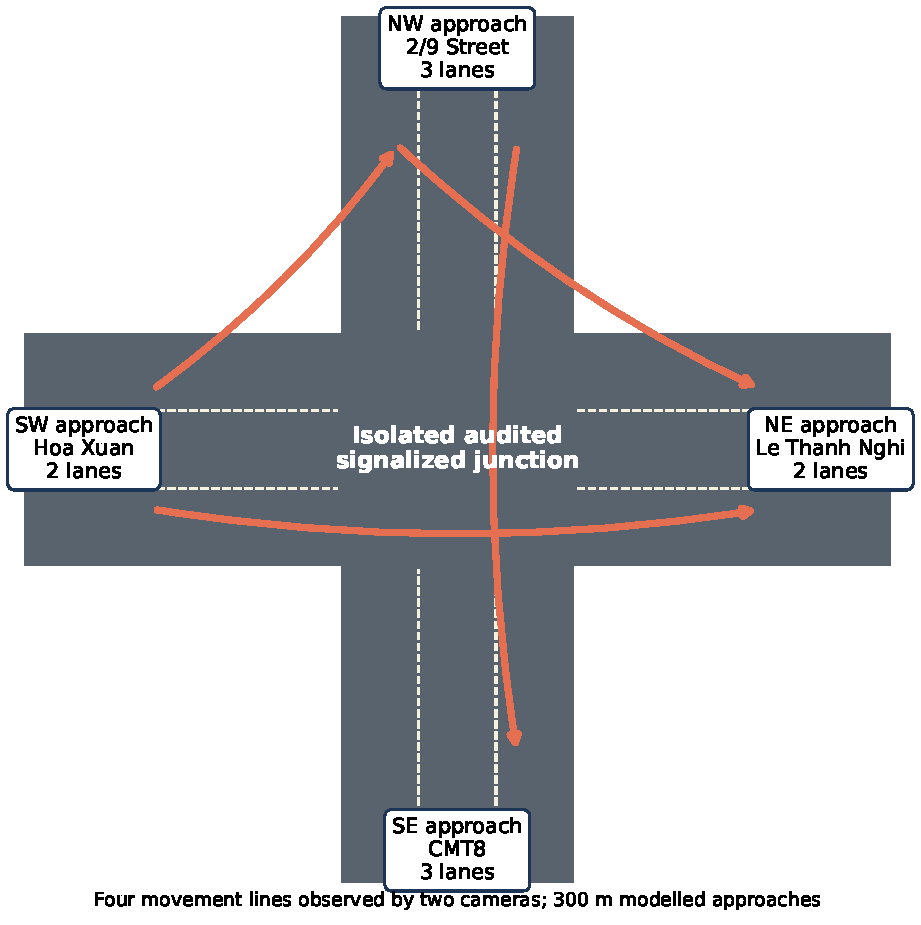
\includegraphics[width=0.82\textwidth]{junction-schematic.pdf}
\caption{Audited isolated junction and the four directly observed movement lines. The schematic simplifies geometry for explanation; the SUMO network is the executable source.}\label{fig:junction}
\end{figure}

An initial full OSM conversion was tested for an hour. It produced confounding queues at nearby nodes, short edge fragments, and 14--21 collisions depending on case. Without validated neighboring signal programs and demand, those failures could not be attributed to the target controller. The full graph remains an audit artifact; the isolated network is the primary experiment.

\section{Observed demand}
Two published camera views yield four digitized movement series, divided into motorcycles, cars, trucks, and buses. The source paper states that camera records were collected from 06:00 to 18:00 on 1 April 2025~\cite[p.~16]{phan2025danang}. The retained CSV contains twelve plotted labels, 07:00 through 18:00, for each of four movements (48 rows). The legacy column name \texttt{hour\_start} is treated as a plot label; the article does not establish the precise timestamp convention for an hourly aggregation window. Counts are read from its Figures 17--18 with an explicit per-series digitization uncertainty of 15 or 30 vehicles per hour. The separate twelve-movement table is reported from 2022 traffic-volume data. The paper attributes it to the transport authority and reference 33, a 2024 planning document that was not independently obtained here. Its explicit proportional estimation statement concerns the 2025 camera-derived directions (pp.~16, 20--21); it does not identify measured versus estimated rows of the 2022 table. The CSV retains a conservative legacy mixed-provenance label, which must not be read as proof that particular Table 1 rows were estimated. The selected camera-supported hours are shown in Table~\ref{tab:demand} and Figure~\ref{fig:profile}.

\begin{table}[H]
\centering
\caption{Camera-derived scenario inputs; approximate counts for four movement lines.}\label{tab:demand}
\small
\resizebox{0.92\textwidth}{!}{%
\begin{tabular}{llllr}
\toprule
Scenario & Local time & Role & Evidence status & Vehicles/hour \\
\midrule
Normal & 13:00 & Held-out test & Four digitized camera movements & 1,395 \\
AM peak & 08:00 & Train/validation/test profile & Four digitized camera movements & 2,330 \\
PM peak & 17:00 & Held-out test & Four digitized camera movements & 2,400 \\
\bottomrule
\end{tabular}
}
\end{table}

\begin{figure}[H]
\centering
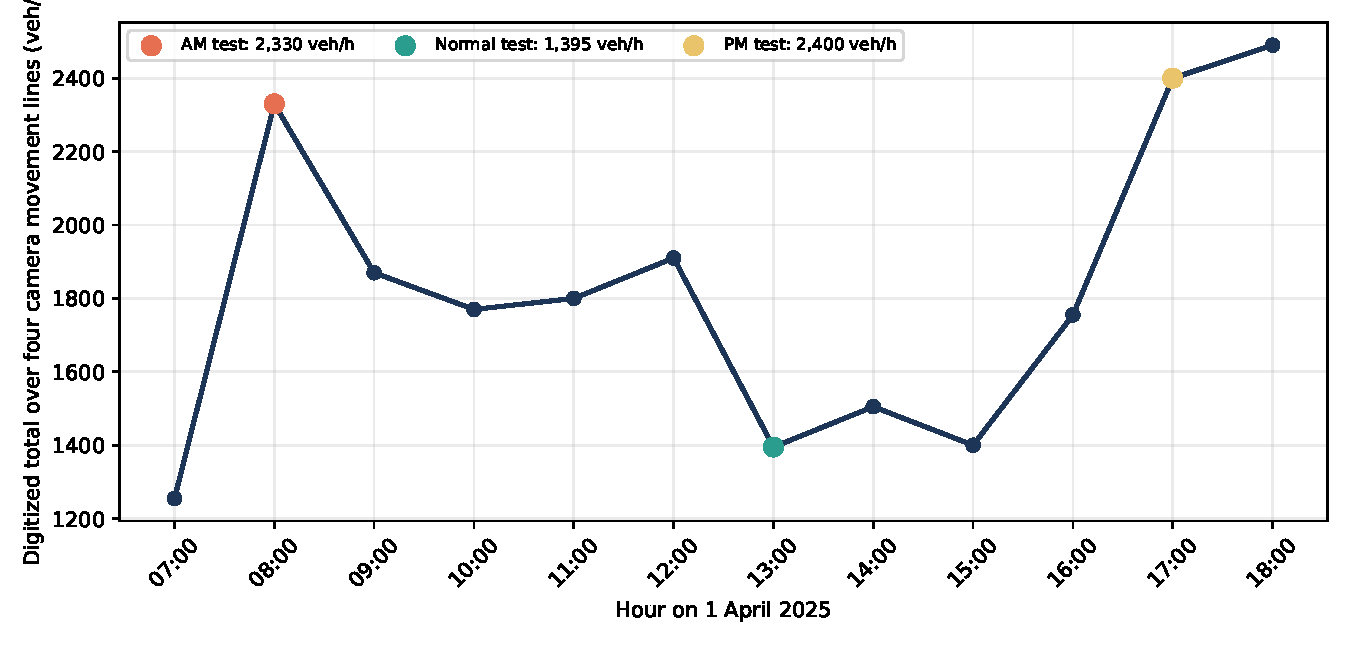
\includegraphics[width=0.93\textwidth]{camera-profile.pdf}
\caption{Digitized sum across the four camera movement lines on 1 April 2025. This is partial intersection coverage, not total city or full-junction traffic.}\label{fig:profile}
\end{figure}

The twelve published peak movements sum to 6,171 PCU/h. Applying observed class mix to all twelve would schedule 5,793, 9,676, and 9,967 vehicles for the three regimes. Those figures are model estimates and are never labeled observed. They are excluded from the primary comparison because their class composition and hourly scaling cannot be independently verified.

\section{District topology and synthetic network demand}
The scale experiment begins from a pinned OpenStreetMap extract and produces a CityFlow road network with 53 controlled signals. The executable roadnet, ordered agent IDs, legal green phases, lane movements, and a separate viewer projection are recorded with SHA-256 hashes. The conversion keeps passenger-vehicle edges and removes residential streets (OSM \texttt{highway.residential}), so the controlled signals lie on the arterial network, consistent with the arterial focus of earlier local coordination work~\cite{tran2007greenwave}. OpenStreetMap supplies topology and coordinates; it does not establish that every mapped node is an operational signal, nor does it supply field timing plans.

Synthetic route families connect boundary entry and exit roads through deterministic metric-shortest valid paths that cross at least two controlled signals. When fewer than three such families reach a controlled signal, the generator adds simple signal-constrained paths no longer than 1.25 times the metric-shortest path for that OD. Coverage-aware set cover seeds the disjoint training, validation, and test pools (50/25/25) and each seeded case; generation fails if any of the 53 controlled signals remains inactive. The manifest reports signal coverage, OD diversity, and route-length distributions for every case. Each case samples 500 route streams from its assigned pool. Three consecutive twenty-minute bins use the relative shape of published normal, AM-peak, or PM-peak camera profiles to set departure intervals, with a 90\% motorcycle share as an explicit modelling assumption. This transfers temporal demand evidence into a reproducible stress generator; it does not turn four observed movement lines into district OD observations.

The immutable experiment manifest contains 30 cases: nine training cases from three demand seeds across all three regimes, six validation cases from two disjoint seeds across the same regimes, and fifteen held-out test cases from five demand/simulator seed pairs across the three regimes. Case files record scheduled vehicle counts, flow hashes, route-family hashes, simulator seeds, and the evidence label. Training and checkpoint selection use their assigned partitions. The bounded controller comparison evaluates the fifteen test cases after checkpoint selection; subsequent design of the PM-only gate used those outcomes and is therefore post hoc.

\section{Vehicle and signal assumptions}
Vehicle classes preserve the published categories. Passenger-car-equivalent weighting is used only to interpret the aggregate movement table; the simulator represents explicit vehicles. The published fixed program contains three green phases and three seven-second clearances, totaling 103 seconds. The adaptive agent acts every ten seconds, must retain green for at least twenty seconds, and automatically traverses the seven-second modelled clearance when a phase changes.

The study initially used a 1.0-second motorcycle time headway. A held-out AM realization produced a rear-end collision at simulation time 1,762 seconds. A one-parameter reproduction showed that 1.2 seconds removed the event. Because headway changes capacity and policy dynamics, all prior checkpoints and results were invalidated and the complete protocol was rerun. This correction is a disclosed development intervention. Because a held-out case informed the headway change, rerunning the same cases does not restore a completely untouched confirmatory test set. The reported outcomes are conditional on the corrected simulator; independent post-correction cases remain necessary for confirmation.

\section{Public-camera counting feasibility demonstration}\label{sec:camera}
The demand evidence above is limited by access: the raw video behind the published camera counts is not public. A separate demonstration therefore tests whether counts and turning movements can be extracted automatically from a public Da Nang traffic camera. Its outputs are called \emph{public-camera YOLO counts} to distinguish them from the digitized published camera counts used in the SUMO tier. They supply no input to either simulator.

\textbf{Source.} The 0511.vn camera at the Tay Cau Rong junctions (J1 and J2 on Nguyen Van Linh, at the west end of the Dragon Bridge) is republished on the public YouTube channel @0511.VietNam.\footnote{\url{https://www.youtube.com/watch?v=31Fhtgcq_fc}; 0511.vn permits non-commercial use with attribution.} The recording is titled as an afternoon of 1/07/2026, whereas the burned-in overlay shows 11 July 2026; as with the junction-name discrepancy above, this thesis follows the overlay and records the inconsistency. The analysed window is 17:15:59--17:30:59 on the overlay clock, fifteen minutes of the evening peak, at 720p and 30 frames per second.

\textbf{Pipeline.} A YOLOv8x detector fine-tuned on the drone-view VisDrone data~\cite{zhu2022visdrone} runs at input size 2,560 and confidence 0.15.\footnote{Ultralytics YOLOv8, \url{https://github.com/ultralytics/ultralytics}; VisDrone weights \url{https://huggingface.co/mshamrai/yolov8x-visdrone}.} A COCO-trained detector found almost no motorcycles from this camera height. VisDrone labels a rider separately from the motorcycle, so the motor, bicycle, tricycle, pedestrian, and people classes are all merged into one motorcycle class, and boxes nested inside another box (a rider on a bike) are removed. ByteTrack~\cite{zhang2022bytetrack} keeps vehicle identities at 10 processed frames per second. Seven count lines record each track once per line and direction, and a track's class is its confidence-weighted vote over its life. Consecutive entry and exit crossings of one track give its turning movement at a junction, and the two junctions are chained through their connecting link as an absorbing Markov chain of $P(\text{exit leg}\mid\text{entry leg})$. Volumes always come from line counts; completed routes supply proportions only.

\begin{figure}[tbp]
\centering
\begin{subfigure}[t]{\textwidth}
\centering
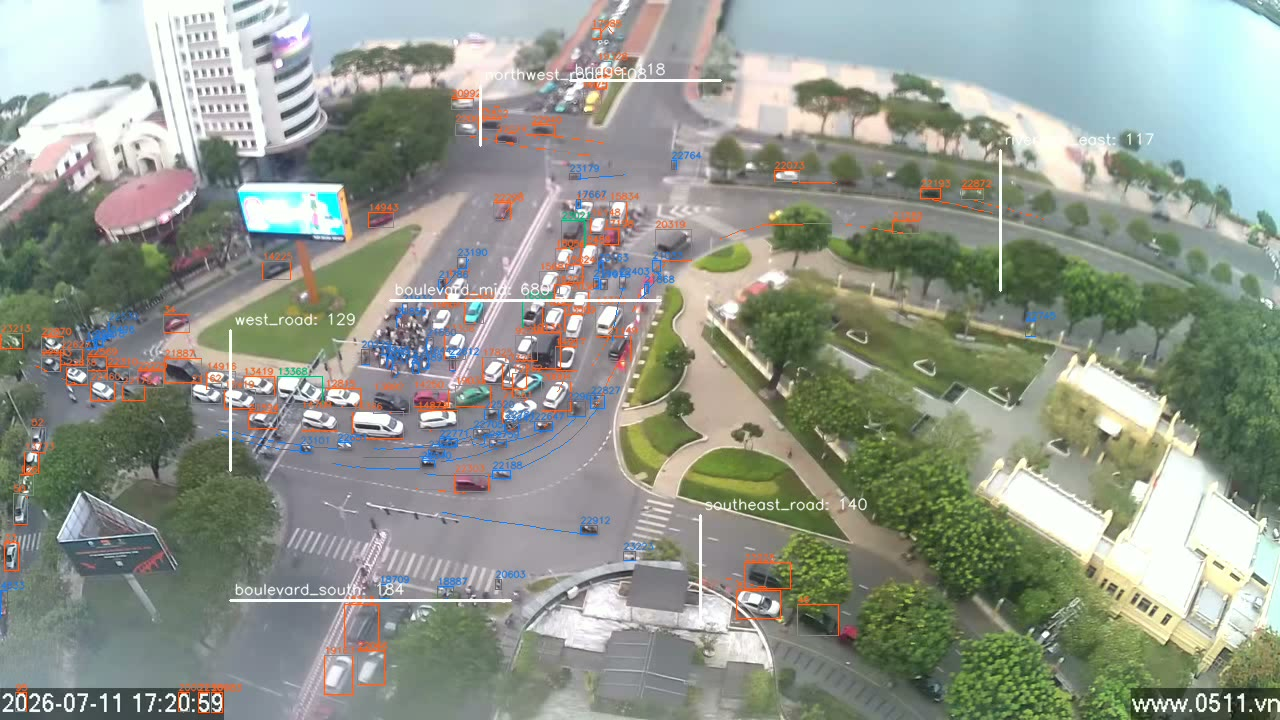
\includegraphics[width=0.62\textwidth]{../results/camera_counts/caurong_20260711_1716/camera_annotated_frame.jpg}
\caption{Detections, track identities, and count lines.}
\end{subfigure}\\[4pt]
\begin{subfigure}[t]{\textwidth}
\centering
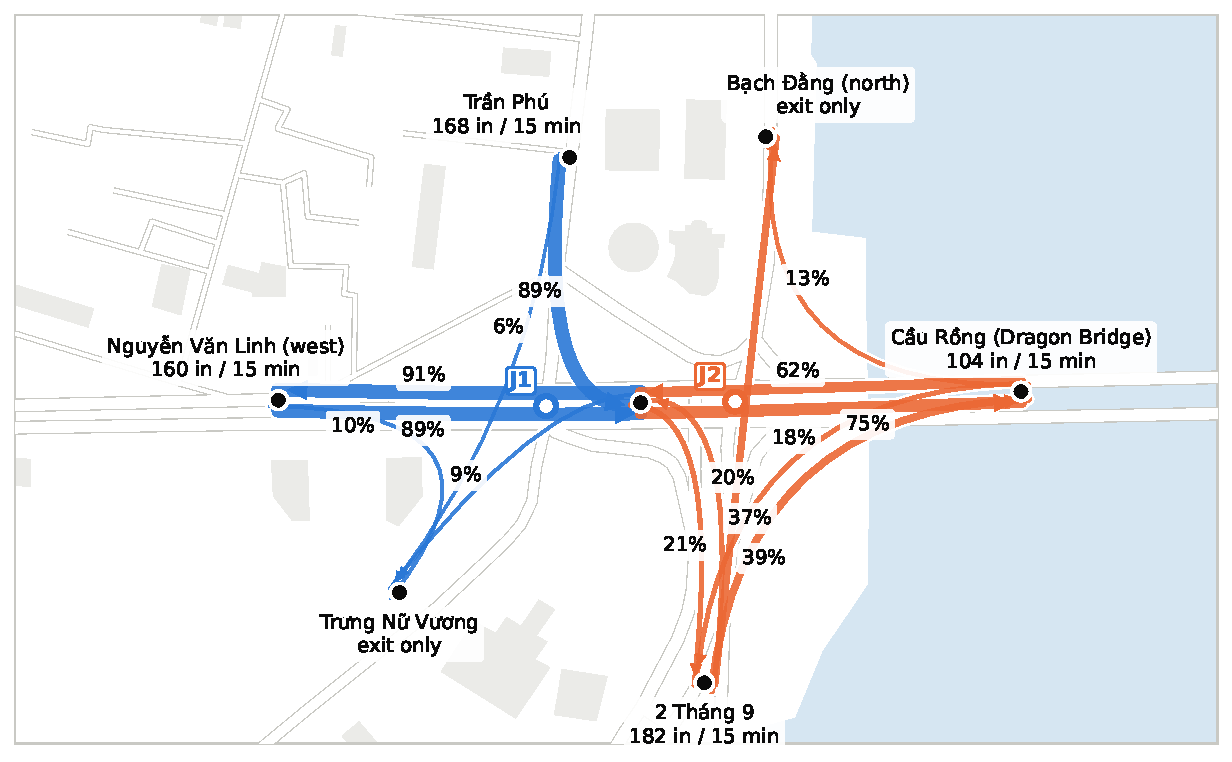
\includegraphics[width=0.7\textwidth]{../results/camera_counts/caurong_20260711_1716/only_car/markov_map_bare.pdf}
\caption{Car turning probabilities at J1 (blue) and J2 (orange).}
\end{subfigure}
\caption{Public-camera counting demonstration at Tay Cau Rong, 11 July 2026, 17:16--17:31. Camera image from 0511.vn; base map \textcopyright{} OpenStreetMap contributors. Arrows below 5\% are hidden.}\label{fig:camera}
\end{figure}

\textbf{Results.} The fifteen minutes contain 4,323 line crossings: 2,420 motorcycles, 1,873 cars and vans, 11 trucks, and 19 buses. On the near-field link between the junctions, which is the most reliable view, the pipeline counts 1,010 motorcycles and 323 cars northbound and 517 motorcycles and 152 cars southbound. Car counts are internally consistent: 480 cars enter J1 and 501 leave it, and 612 enter J2 and 735 leave it, gaps of 4\% and 17\%. For 689 car entries (63\%), the same track is later seen leaving, giving a completed route. Of the cars arriving at J2 along the link, 75\% (154 of 204) continue onto the Dragon Bridge, and through the chain 68\% of cars entering J1 from either Tran Phu or Nguyen Van Linh (west) end on the bridge (Figure~\ref{fig:camera}). The approaches counted in one direction only match the one-way tags in OpenStreetMap, an independent plausibility check.

\textbf{Real-time operation.} With a smaller YOLOv8m model at input size 1,280 and 7.5 processed frames per second, the full pipeline, including model loading, processed 180 seconds of video in 169 seconds on one Apple M4 Pro laptop. Detection takes about 68~ms per frame, far below the 10-second SUMO decision interval. On the same 180 seconds the faster settings counted near-field cars at $+8\%$ (194 versus 180) and near-field motorcycles at $-10\%$ (394 versus 439) relative to the reference run. A 53-signal deployment would need one such pipeline per junction; that scale was not tested.

\textbf{Limits.} No manual count exists yet, so detection and identity accuracy are unmeasured. Far-field motorcycles are badly under-counted: 174 enter the observed cordon while 703 leave it. Motorcycle totals at the cordon are therefore lower bounds, and motorcycle turning proportions are not reported. Because pedestrian and bicycle classes are merged into the motorcycle class, a pedestrian or cyclist crossing a count line is counted as a motorcycle. The evidence is one camera, one date, and fifteen minutes at a junction different from the SUMO anchor. The annotated video stays local. The demonstration shows that measured counts and turning probabilities are obtainable from public infrastructure; it does not calibrate either simulator.

\chapter{Methodology}\label{ch:method}
This chapter specifies the controllers and protocols that make up \methodname{}: the single-junction decision process, learning algorithm, baselines, and split, followed by the network extension.

\section{Single-junction Markov decision process}
At decision time $t$, the state is a 16-dimensional vector: for each of the four approaches, the stopped queue, the number of vehicles on the approach, and the vehicles waiting to enter the network, plus a one-hot encoding of the three green phases and the time since the last switch (capped at 60 seconds and scaled to $[0,1]$). Counts are normalized by 20. The action $a_t\in\{0,1,2\}$ selects one of the three admissible green phases. Signal safety logic may delay an action through the clearance interval and minimum-green rule.

The one-step reward is the negative total queue:
\begin{equation}
r_t=-0.01\left(q_t^{\mathrm{network}}+q_t^{\mathrm{pending}}\right).
\end{equation}
Including pending vehicles prevents a controller from appearing successful by blocking insertion at the model boundary. The primary episode outcome is the exact one-second integral
\begin{equation}
\qint=\frac{1}{3600}\sum_{t=1}^{3600}
\left(q_t^{\mathrm{network}}+q_t^{\mathrm{pending}}\right),
\end{equation}
reported in vehicle-hours.

\section{Single-junction learning algorithm}
The replay tuple is $(s_t,a_t,R_t^{(3)},s_{t+3},d_t)$. The three-step return is
\begin{equation}
R_t^{(3)}=r_t+\gamma r_{t+1}+\gamma^2r_{t+2}, \qquad \gamma=0.99.
\end{equation}
The Double DQN target uses the online network to choose the action and the target network to evaluate it. A Huber loss and gradient clipping at 10 control extreme updates. Experience replay begins after 256 decisions; minibatches contain 64 samples; the target network synchronizes every 200 optimization steps. Exploration decays linearly from 1.0 to 0.05 over 5,000 decision steps.

The network has two fully connected 64-unit hidden layers followed by dueling value and advantage heads. Each training run contains thirty full one-hour episodes. Every fifth episode, a greedy full-hour validation is executed on the separate validation departure realization. The checkpoint with the smallest validation mean queue is frozen.

\section{Single-junction baselines and ablation}
The published fixed-time plan is the principal baseline because it is the historical plan reported for the site. Raw Max-Pressure chooses the largest estimated approach pressure at every admissible decision. Hysteretic Max-Pressure changes phase only when the alternative exceeds the current phase by a margin. A base Double DQN without dueling heads and using one-step returns is trained at seed 11 under the same budget. This architecture ablation tests the combined dueling/three-step change; it is not a full factorial attribution.

\section{Single-junction protocol and independence}
Table~\ref{tab:split} defines the split before held-out evaluation. Departure generation preserves the exact class and movement counts while changing within-hour timing. Hashes in the experiment manifest prove that the realizations differ.

\begin{table}[H]
\centering
\caption{Data and randomization split.}\label{tab:split}
\begin{tabularx}{\textwidth}{l>{\raggedright\arraybackslash}Xll}
\toprule
Partition & Demand profile & Demand seeds & Simulator/learning seeds \\
\midrule
Training & AM peak & 11 & simulator 11; learning 11--15 \\
Validation & AM peak & 31 & simulator 31, shared by all runs \\
Held-out test & Normal, AM, PM & 101--105 & simulator 201--205 \\
Sensitivity & AM scaled 0.75--1.50 & 101--105 & frozen policies only \\
\bottomrule
\end{tabularx}
\end{table}

The five DDQN policies are independent learning replicates. Each is crossed with the same fifteen held-out demand cases. Therefore, the analysis first averages cases within each training seed; it never treats 75 correlated DDQN evaluations as 75 independent policies. Fixed-time confidence intervals use five demand realizations per scenario. Paired DDQN-minus-fixed effects match on demand realization, average within training seed, and bootstrap those five seed-level effects with 20,000 resamples.

\section{Hai Chau network extension protocol}
The completed analysis uses the 53-signal topology, thirty-case manifest, and matched 3,600-second cases described above. Its evidence tier is bounded and exploratory. A separate strict release protocol exists in the software but has not completed. Planning reports provide context only~\cite{jica2014tiensa,dacriss2010danang}; they supply no district OD calibration.

\subsection{Controller identity and schedule contract}\label{sec:residual}
The evaluated learned controller is \texttt{schedule\_residual\_ddqn}. It scores bounded changes to a validation-tuned 25-second fixed-time reference. Normal mode executes that reference exactly. At 300-second macro boundaries in peak mode, a candidate either retains the reference or shifts one request boundary by $\pm10$ seconds. A compiler masks infeasible changes and requires the executed signal state to rejoin the reference at the block end. The simulation action interval is 10 seconds, with configured minimum green 20 seconds and maximum red 180 seconds; transition semantics also depend on the source-bound phase contract. A configured three-second yellow parameter does not establish that every source transition lasts exactly three seconds. These are executable modelling constraints, not a field safety certificate.

Each macro has 27 features: twelve features for its source phase, twelve for its target phase, and three macro descriptors (boundary fraction, shift fraction, and baseline indicator). The phase features include local queues, downstream remaining capacity, and mean upstream/downstream neighbor queues. One shared scalar-scoring network with two 64-unit hidden layers serves all signals. It uses Double DQN targets, without dueling value/advantage heads. The twelve-episode training budget, checkpoints at episodes 4/8/12, and exact optimizer values are taken from retained resolved configurations, not from a later candidate YAML file.

The macro reward is the negative increment of network-plus-pending queue integral. Stored rewards retain vehicle-seconds; the critic scales them by 100,000 for numerical units. The semi-Markov target discounts by $\gamma^{\Delta t/300}$, with $\gamma=0.99$. It is not the three-step return of the single-junction dueling agent, nor the older phase-scoring queue/blocking/switch weighted reward. The relevant code is \path{src/traffic_rl/agents/schedule_residual.py}; the seed-14 configuration and contract are preserved in \path{docs/research/evidence-snapshot-2026-09-23/}.

Neighbor features provide local context. Their causal benefit is not isolated by the completed network matrix: no matched multi-seed removal of neighbor features or shared-vector ablation is reported. Operation across 53 signals demonstrates execution at that scale, not a measured scaling law or citywide coordination benefit.

\subsection{Baselines and selection outcomes}
The completed four-controller matrix contains tuned fixed-time, Max-Pressure, hysteretic Max-Pressure, and residual DDQN at seed 14, episode 4. Fixed-time is selected from green durations 20, 25, 30, 35, 40, 45, 50, and 60 seconds using the six validation cases. The three baselines and the learned controller use matched case inputs. The fifteen-case matrix is a single-policy comparison; its case bootstrap cannot estimate variation across independent learning seeds.

Residual checkpoints at episodes 4, 8, and 12 are evaluated using validation gates for exact normal-mode fallback, peak queue regret, insertion/completion loss, nonzero learned activity, and schedule validity. The retained selection records mark seeds 12, 14, and 15 as selected at episodes 8, 4, and 8. Seeds 13 and 16 are rejected and have no selected winner. Their later episode-12 and episode-4 diagnostic replays may contribute to exploratory analysis only. The earlier V3-A schedule-rehearsal and no-rehearsal phase-scoring pilots were also rejected; their design must not be presented as the controller behind the residual result.

\subsection{Post hoc regime gate and statistical unit}
After inspecting residual test behavior, the exploratory gate retains fixed-time in normal and AM conditions and uses residual DDQN in PM. The regime is supplied as declared operational context; the experiment does not evaluate a learned regime detector, detection errors, or transitions between regimes. Cases are separate one-hour episodes from reset. Seeds 13 and 16 combine fresh fixed normal/AM replays with fresh residual PM replays; they do not represent continuous full-day operation.

For seed $s$, the pooled reduction is
\begin{equation}
I_s=100\frac{\sum_{c=1}^{15}Q_{F,c}-\sum_{c=1}^{15}Q_{s,c}}
{\sum_{c=1}^{15}Q_{F,c}}.
\end{equation}
The reported 3.48\% is the mean of these five seed-level ratios; its percentile bootstrap resamples the five values 10,000 times with random seed 20260913. It is conditional on the same fifteen cases and the post hoc gate. It neither corrects selection bias nor quantifies uncertainty across independent traffic days. The fifty normal/AM seed-case cells are exact fixed-time ties by construction; only the twenty-five PM cells can express a learned effect. Case regressions must therefore be reported alongside the aggregate. Ratio-of-sums reductions and unweighted means of case percentages are explicitly distinguished.

\subsection{Confirmation and robustness still required}
A confirmatory study must freeze its controller, regime rule, eligible checkpoints, baselines, metrics, and analysis before evaluating new demand realizations unused in development. Replaying the already inspected fifteen cases is not a new independent test. Failed seed selections must be reported under the frozen rule; they cannot be replaced by favorable diagnostic checkpoints after test inspection.

The repository also contains a planned robustness appendix: demand $+20\%$, sensor noise, sensor dropout, and a lane restriction. Its proposed matrix has 420 fresh episodes. No completed 420-episode result for the current residual/gated controller is claimed here. Legacy robustness outputs belong to different protocols. The current thesis reports completed demand-scale sensitivity at the single junction; network robustness remains future work. Passing an artifact verifier would establish protocol consistency, not field validity or automatic statistical superiority.

\chapter{Implementation and Verification}\label{ch:implementation}

\section{Software architecture}
The two evidence tiers use separate simulator stacks and configuration namespaces, summarized in Table~\ref{tab:software-stacks}. They share Python orchestration, NumPy learning code, immutable manifests, and the rule that training, evaluation, summarization, figure generation, and demo export are separate commands.

\begin{table}[H]
\centering
\caption{Software and configuration boundaries for the two experiments.}\label{tab:software-stacks}
\small
\begin{tabularx}{\textwidth}{p{2.7cm}p{4.0cm}>{\raggedright\arraybackslash}X}
\toprule
Experiment tier & Runtime & Bound inputs and outputs \\
\midrule
Empirical anchor & SUMO controlled through TraCI; Python/NumPy learner & Isolated network and route XML, published signal program, explicit vehicle parameters, departure hashes, collision/emergency-braking records, \texttt{danang\_protocol\_v1} results \\
District scale & Digest-pinned CityFlow Python-3.6 container; Python/NumPy shared learners & 53-signal roadnet and phase-contract hashes, 30 flow files, resolved controller and reward configuration, checkpoint contracts, per-run manifests, \texttt{haichau\_network\_v2} results \\
\bottomrule
\end{tabularx}
\end{table}

The SUMO environment exposes queue state, applies the published seven-second modelled clearance, records collisions and emergency braking, and checks accounting identities among scheduled, inserted, running, arrived, and pending vehicles. The CityFlow path represents every controlled node through one ordered 53-agent manifest. Its release runner materializes and hashes the complete resolved run configuration before inspecting or invoking Docker, records the project mount and working directory, disables container networking, and retains canonical logs and runtime identity for audit. Final evaluation consumes frozen checkpoints and case bytes; it has no training path.

\section{Verification gates}
For the empirical anchor, automated tests cover the published 103-second program, four-approach network, observed counts, demand realization hashes, vehicle classes, full-hour rear-end regression, split separation, exact queue integral, controller safety constraints, checkpoint loading, and seed-aware statistics. For the strict district-scale release, gates additionally verify exactly 53 ordered agents, disjoint route families, all 30 case hashes, a digest-pinned CityFlow runtime, the hash-bound V3 selector, five eligible learned checkpoint bundles, fresh matched runs for all four controllers, complete horizons and vehicle identities, hierarchical statistics, generated paper artifacts, six offline replays, decoded fallback media, and a clean-checkout attestation. The confirmatory release is releasable only when every gate passes in one final report. The bounded result reported below is a separate, explicitly labelled evidence tier.

\section{Accounting and safety}
At every run end, the evaluator records scheduled, inserted, arrived, running, pending, collision, and emergency-braking totals. Pending demand is included in the queue integral. All primary held-out runs use the final 1.2-second motorcycle headway. The simulation uses collision output as a required metric instead of relying on console warnings.

\chapter{Results}\label{ch:results}

\section{Training and architecture selection}
For seed 11, the base DQN reaches a best validation mean queue of 81.43 vehicles; the dueling three-step version reaches 71.71 under the same thirty-episode budget. The combined modification is therefore selected for the five-seed experiment. Across the selected architecture, best validation queues are 71.71, 73.07, 87.26, 70.25, and 83.74 for seeds 11--15. The spread is material and persists into held-out performance.

\begin{figure}[H]
\centering
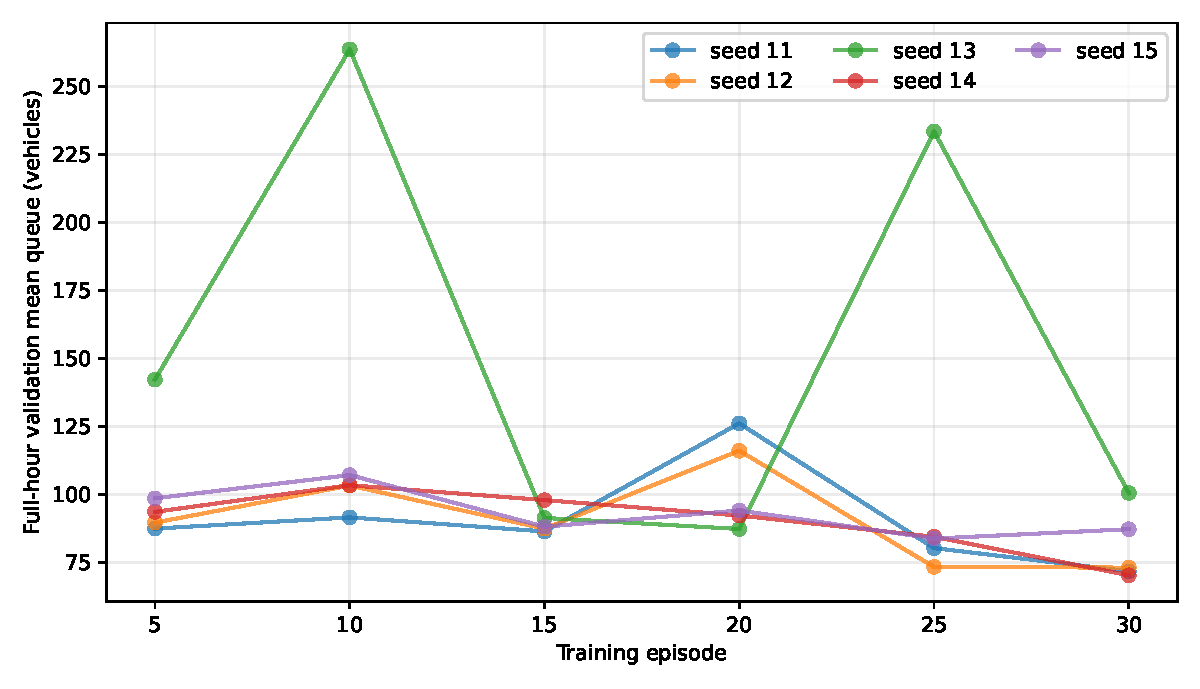
\includegraphics[width=0.88\textwidth]{validation-learning-curves.pdf}
\caption{Full-hour greedy validation during training. Non-monotonic curves and between-seed variation motivate checkpoint selection and seed-level uncertainty.}\label{fig:learning}
\end{figure}

\section{Primary controller comparison}
Table~\ref{tab:primary} reports the stopped-plus-pending queue integral. Lower is better. DDQN is summarized over five independent learned policies; each policy value is its average over five matched demand realizations.

\begin{table}[H]
\centering
\caption{Primary held-out queue integral in vehicle-hours, mean [95\% bootstrap CI].}\label{tab:primary}
\resizebox{\textwidth}{!}{%
\begin{tabular}{lrrr}
\toprule
Controller & Normal 13:00 & AM peak 08:00 & PM peak 17:00 \\
\midrule
Published fixed & 9.86 [9.73, 9.94] & 79.20 [75.90, 83.28] & 152.67 [147.69, 157.04] \\
Raw Max-Pressure & 140.72 & 352.43 & 269.02 \\
Hysteretic MP & 126.85 & 281.52 & 241.40 \\
Dueling DDQN & 41.50 [17.46, 66.01] & 78.41 [69.74, 87.70] & 99.97 [83.12, 117.32] \\
\bottomrule
\end{tabular}
}
\end{table}

\begin{figure}[H]
\centering
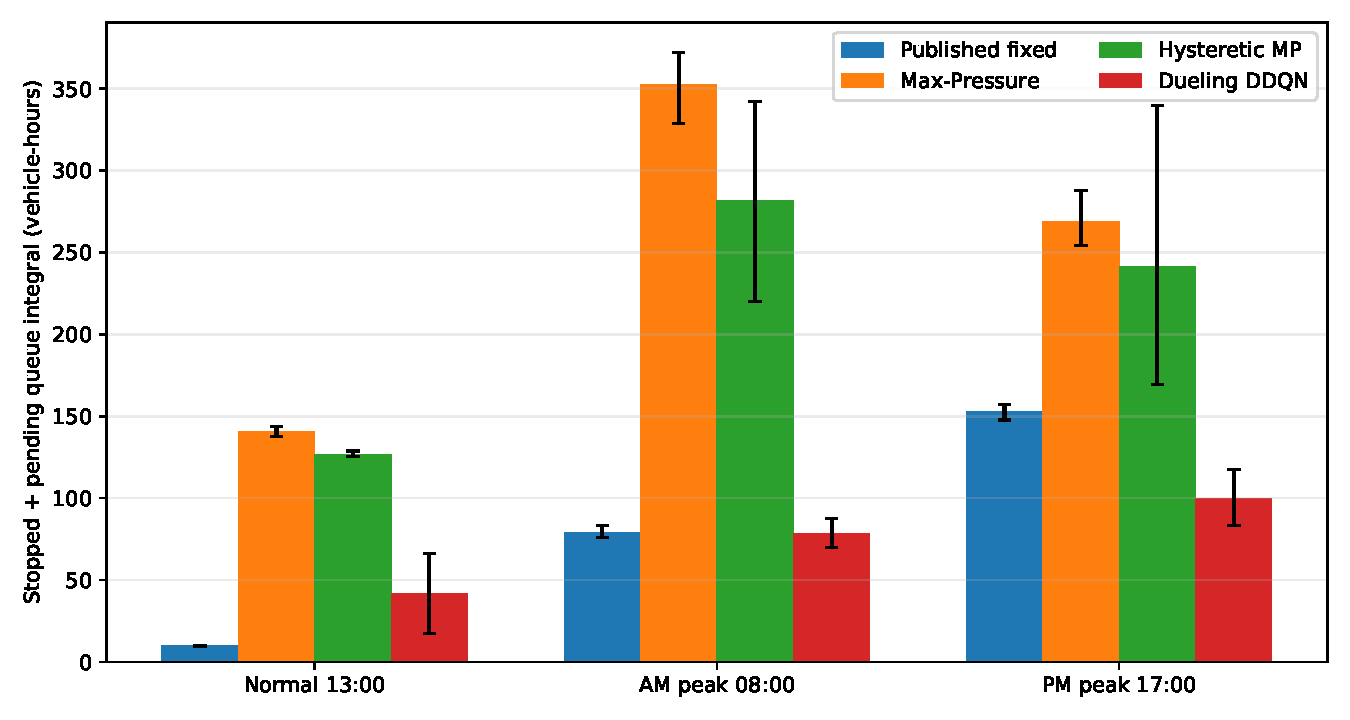
\includegraphics[width=0.95\textwidth]{controller-comparison.pdf}
\caption{Held-out controller comparison. Error bars represent the appropriate independent unit for fixed time and learned policies.}\label{fig:comparison}
\end{figure}

The paired DDQN effect relative to fixed time is $+31.63$ vehicle-hours in normal traffic, equivalent to $+320.7\%$ and therefore harmful. Its 95\% interval is $[7.60,56.14]$. At the AM peak the effect is $-0.80$ vehicle-hours ($-1.0\%$), with interval $[-9.47,8.49]$; the experiment does not resolve a difference and does not establish equivalence. At the PM peak, DDQN reduces the integral by 52.70 vehicle-hours ($34.5\%$), with interval $[-69.55,-35.34]$. All 120 primary held-out controller runs record zero collisions and zero emergency-braking events.

Both Max-Pressure variants perform poorly. This does not refute Max-Pressure theory. The implemented pressure signal sees only partial movements, and seven-second transition loss is substantial relative to a ten-second decision interval. Raw MP changes too readily; hysteresis helps but remains worse than the published plan. The negative result shows that a theoretically strong baseline still requires compatible observation and phase definitions.

\section{Baseline ranking across 1,000 demand realizations}
The fixed-time and Max-Pressure values in Table~\ref{tab:primary} rest on five demand realizations per regime. To test whether that ranking depends on the particular test cases, the three non-learning baselines were rerun on 1,000 additional realizations per regime, 9,000 one-hour SUMO runs in total. Realization $k$ uses demand seed $100000+k$ and SUMO seed $200000+k$, disjoint from all training, validation, and test seeds, and all three baselines run on the same pair, so comparisons are paired. As in the protocol, each realization preserves the observed class and movement counts and redraws within-hour departure times. A parity check first reproduced the held-out AM case with demand seed 101 exactly. The learned controller is not included because each realization would require evaluating all five trained policies; its results remain those of Table~\ref{tab:primary}.

\begin{table}[H]
\centering
\caption{Baseline queue integral over 1,000 paired demand realizations per regime, median [2.5th, 97.5th percentile] in vehicle-hours, and paired win counts.}\label{tab:mc}
\resizebox{\textwidth}{!}{%
\begin{tabular}{lrrr}
\toprule
 & Normal 13:00 & AM peak 08:00 & PM peak 17:00 \\
\midrule
Published fixed & 9.88 [9.49, 10.29] & 78.47 [69.12, 88.70] & 149.27 [136.28, 161.33] \\
Raw Max-Pressure & 137.92 [132.65, 144.81] & 352.12 [300.36, 396.57] & 249.72 [239.50, 354.22] \\
Hysteretic MP & 126.64 [123.22, 130.47] & 292.95 [144.28, 389.14] & 170.72 [167.54, 348.00] \\
\midrule
Fixed lower than raw MP & 1,000/1,000 & 1,000/1,000 & 1,000/1,000 \\
Fixed lower than hysteretic MP & 1,000/1,000 & 1,000/1,000 & 999/1,000 \\
Hysteretic lower than raw MP & 1,000/1,000 & 758/1,000 & 884/1,000 \\
\bottomrule
\end{tabular}
}
\end{table}

\begin{figure}[H]
\centering
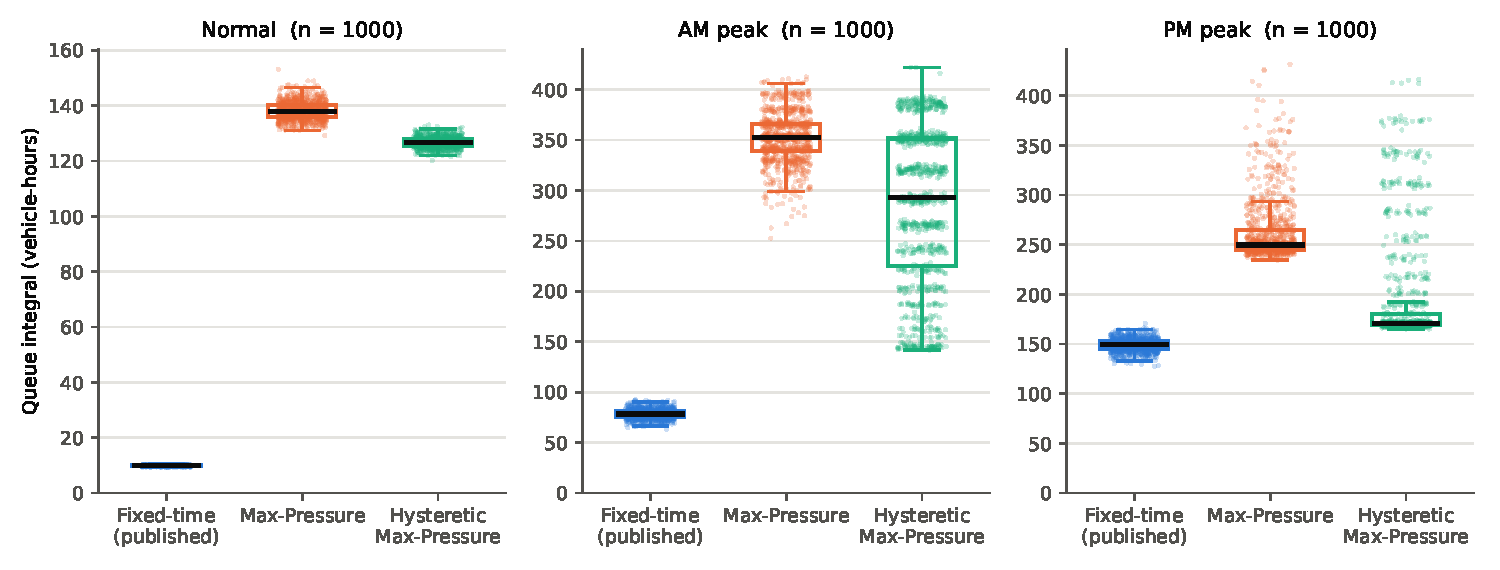
\includegraphics[width=0.95\textwidth]{../results/danang_baseline_mc/baseline-mc-boxplot.pdf}
\caption{Baseline queue integral over 1,000 paired demand realizations per regime. Points are individual realizations; boxes show the quartiles.}\label{fig:mc}
\end{figure}

Table~\ref{tab:mc} and Figure~\ref{fig:mc} show that the ranking is not an artifact of the five test cases. The published plan has a lower queue integral than raw Max-Pressure in all 3,000 paired realizations and than hysteretic Max-Pressure in 2,999 of 3,000. The fixed-time medians, 9.88, 78.47, and 149.27 vehicle-hours, are close to the protocol means of 9.86, 79.20, and 152.67. Hysteresis always helps in normal demand, but at the peaks it beats raw Max-Pressure in only 75.8\% (AM) and 88.4\% (PM) of realizations, and its outcomes split into distinct bands. A plausible explanation is that the hold rule makes the phase sequence path dependent, so small changes in departure timing lock the controller into different switching cycles. Collision counts were not recorded in this batch, so it makes no safety claim. These are realizations of one observed profile per regime, not 1,000 independent traffic days, so they quantify sensitivity to departure timing and simulator randomness, not day-to-day variation in Da Nang traffic.

\section{Demand sensitivity}
The frozen fixed and DDQN controllers are evaluated at four multipliers of the observed AM profile. The 1.00$\times$ level uses the camera-derived AM counts; all departures are simulated, and other multipliers are synthetic sensitivity cases. The thirty outcomes at 1.00$\times$ repeat the primary AM conditions and are not additional independent evidence. Table~\ref{tab:sensitivity} and Figure~\ref{fig:sensitivity} show a crossover between low and congested demand.

\begin{table}[H]
\centering
\caption{Synthetic AM demand sensitivity, queue integral in vehicle-hours.}\label{tab:sensitivity}
\begin{tabular}{rrrrr}
\toprule
Scale & Scheduled veh. & Fixed mean & DDQN mean & DDQN change \\
\midrule
0.75 & 1,747 & 13.95 & 39.21 & +181.2\% \\
1.00 & 2,330 & 79.20 & 78.41 & -1.0\% \\
1.25 & 2,913 & 307.16 & 159.11 & -48.2\% \\
1.50 & 3,495 & 595.67 & 389.10 & -34.7\% \\
\bottomrule
\end{tabular}
\end{table}

\begin{figure}[H]
\centering
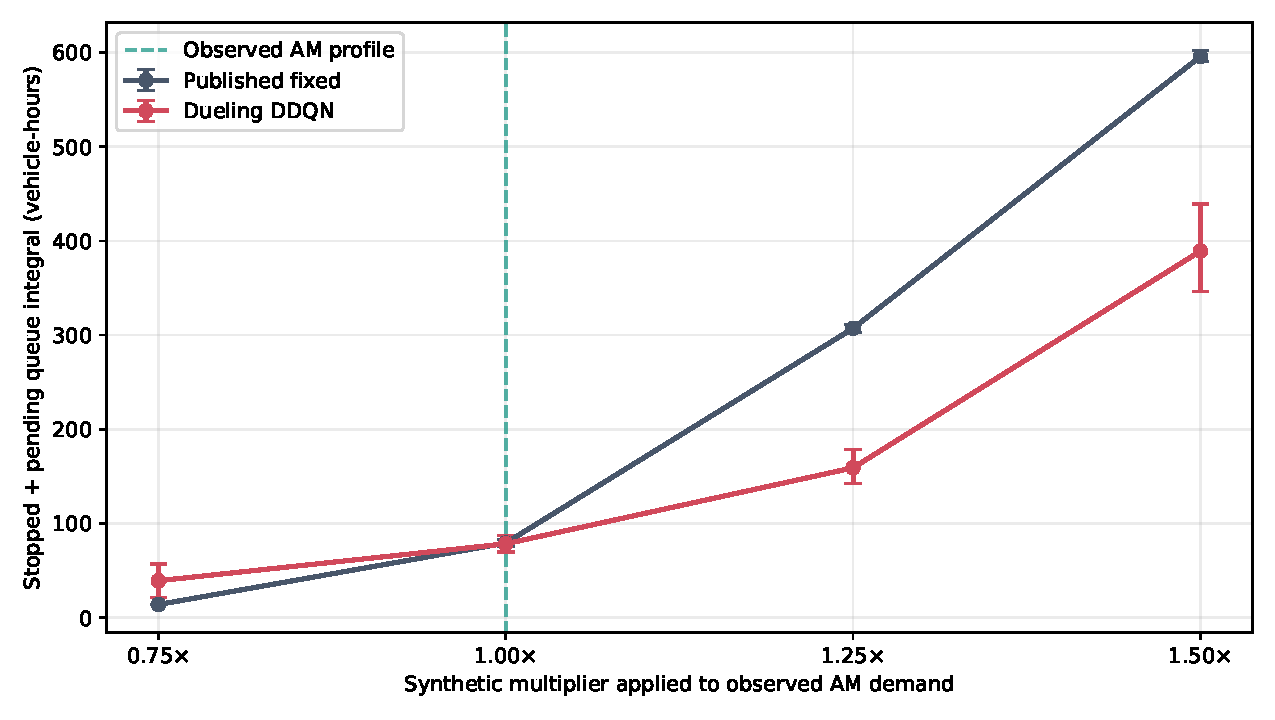
\includegraphics[width=0.9\textwidth]{demand-sensitivity.pdf}
\caption{Demand sensitivity of frozen controllers. The dashed line marks the observed AM profile; other levels are synthetic.}\label{fig:sensitivity}
\end{figure}

No collision occurs in the 120 sensitivity runs. Four emergency-braking events are recorded. Their rarity does not validate real-world safety, but retaining them prevents a zero-event primary table from hiding a model warning under stress.

\section{Current Hai Chau network bounded result}
The preceding tables report the completed single-junction SUMO study. To make the current 53-signal implementation auditable while the
five-seed release gate is still pending, we ran a bounded held-out comparison
using the final seed-14, step-4 schedule-residual DDQN checkpoint. It covers
all fifteen declared test realizations (demand seeds 101--105 in normal,
AM-peak, and PM-peak regimes), with a matched 3,600-second horizon and the
validation-tuned 25-second fixed-time controller. The residual controller is
exactly equal to fixed-time in normal operation by its anchored policy
contract.

Across the fifteen matched cases, fixed-time accumulated 8,339.43
vehicle-hours of queue integral and residual DDQN accumulated 7,829.25, a
6.12\% aggregate reduction. The unweighted means of case-level percentage reductions were 0.00\% in normal demand,
3.53\% in the AM peak, and 8.86\% in the PM peak. The corresponding
ratio-of-sums reductions are 0.00\%, 3.48\%, and 10.39\%, respectively. Case effects ranged from a
4.24\% regression to a 26.11\% improvement, so the aggregate result is
evidence of a measured gain rather than a claim that every realization
improves. A paired bootstrap over case-level effects gives a 95\% interval of
[0.90\%, 8.35\%]. The machine-readable rows and hashes are stored in
\path{results/haichau_network_v2/final15-seed14-step4-summary.json}.

Checkpoint sensitivity is also reported. Seed 12, step 8 over the same fifteen
cases reduced the aggregate metric by only 0.78\% and regressed 5.67\% in the
AM peak; seed 15, step 8 reduced it by 0.44\%, with a paired bootstrap interval
of [$-$3.99\%, 3.99\%]. These weaker and regime-dependent results show why validation selection and
independent confirmation remain necessary. The bounded seed-14 result resolves the
normal-hour failure mode and provides a defensible network-scale result for the
presentation demo, but it does not replace the preregistered five-seed release
campaign or its fail-closed verifier.

At the learning-seed level, the five fresh gated replays have a mean aggregate
improvement of 3.48\% (range 1.03--5.62\%). Normal and AM are exact fixed-time
ties by construction; the PM reductions range from 2.09\% to 11.43\%.
The seed-level bootstrap 95\% interval for the derived pooled-case effects is
[2.01\%, 4.95\%]. This exploratory seed-level result is stored in
\path{results/haichau_network_v2/final15-regime-gated-direct-multi-seed-summary.json};
it does not substitute for the still-pending strict confirmatory release.

The seed sensitivity suggests a demand gate that can be tested without
changing the signal-safety contract: retain tuned fixed-time in normal and AM
peak demand, where the residual learner is least stable, and enable the
residual policy only in PM peak. Composing the completed matched rows under
that rule gives 2.83\% lower queue-hours across 45 rows, with seed-level
reductions of 2.36\%, 5.11\%, and 1.03\% for seeds 12, 14, and 15. This is an
exploratory counterfactual composition rather than a fresh controller run; it
motivates a preregistered gated campaign and is stored in
\path{results/haichau_network_v2/final15-regime-gated-summary.json}.

We then ran the same gate as a direct fresh replay for seed 14 rather than a
row composition. Across all fifteen test cases, fixed-time accumulated 8,339.43
vehicle-hours and the gated controller accumulated 7,913.46, a 5.11\%
reduction. Normal and AM were exact fixed-time ties, while the PM aggregate
reduction was 10.39\%. The direct rows retain the same network, demand hashes,
checkpoint identity, and 3,600-second horizon in
\path{results/haichau_network_v2/final15-regime-gated-seed14-direct-summary.json}.
This is still exploratory evidence because the gated controller is outside the
frozen five-seed release protocol.

The same policy was replayed on the five PM test cases for seed 13. Queue-hours
fell from 4,100.74 to 3,631.89 (11.43\%); one case regressed by 1.76\%, while
the other four improved. Its direct rows are stored in
\path{results/haichau_network_v2/final15-regime-gated-seed13-pm-direct-summary.json}.

A separate PM-only replay for seed 16 produced 3,827.77 vehicle-hours
against 4,100.74 for fixed-time, a 6.66\% aggregate reduction. Two of the five
cases regressed, so this result is reported with its case-level variation and
remains exploratory. Across the direct PM gate replays for seeds 13, 14, and
16, the derived pooled-case aggregate reductions are 5.62\%, 5.11\%, and 3.27\%
(mean 4.67\%). The seed-16 rows are stored in
\path{results/haichau_network_v2/final15-regime-gated-seed16-pm-direct-summary.json}.

Fresh pooled-case gate replays for seeds 12 and 15 cover all fifteen held-out
cases. Their queue-hours fall from 8,339.43 to 8,142.43 (2.36\%) and 8,253.86
(1.03\%), respectively. Normal and AM are exact fixed-time ties; the fresh PM
reductions are 4.80\% and 2.09\%, with case-level regressions. Across the five fresh
seed summaries, the derived pooled-case reductions are 2.36\%, 5.62\%, 5.11\%,
1.03\%, and 3.27\% (mean 3.48\%). All five seeds have fresh fifteen-case
coverage. Seeds 12, 14, and 15 use direct pooled-case gate
campaigns, while seeds 13 and 16 combine fresh fixed normal/AM replays with
fresh PM gate replays. The provenance table is stored in
\path{results/haichau_network_v2/final15-regime-gated-direct-multi-seed-summary.json}.
At the case level, the gate regresses 3/15 cases for seed 12, 1/15 for seed 13,
1/15 for seed 14, 3/15 for seed 15, and 2/15 for seed 16; the positive aggregate
does not imply improvement for every demand realization.

The gate was devised after test inspection. Furthermore, the original validation selector rejected seeds 13 and 16. Their diagnostic checkpoints do not become validation-eligible because a post hoc gate yields a positive aggregate. Thus the five-seed interval describes retained exploratory outcomes and cannot support a five-eligible-seed confirmatory claim. Across the twenty-five PM seed-case cells, fifteen improve and ten regress; the other fifty cells tie fixed-time by construction.

\begin{table}[H]
\centering
\caption{Direct exploratory regime-gated replay by learning seed.}
\label{tab:gated-seed-replays}
\begin{tabular}{lrrrr}
\toprule
Seed & Case coverage & Pooled reduction & PM reduction & Regressions \\
\midrule
12 & 15 cases & 2.36\% & 4.80\% & 3/15 \\
13 & 15 cases & 5.62\% & 11.43\% & 1/15 \\
14 & 15 cases & 5.11\% & 10.39\% & 1/15 \\
15 & 15 cases & 1.03\% & 2.09\% & 3/15 \\
16 & 15 cases & 3.27\% & 6.66\% & 2/15 \\
\bottomrule
\end{tabular}
\vspace{-2pt}
\begin{minipage}{0.92\textwidth}
\small\textit{Note: for seeds 13 and 16, normal/AM are fresh fixed-time replays
and PM is a fresh residual-policy replay; the effective controller is recorded per case. Seeds 13 and 16 were rejected by the original validation selector and remain diagnostic.}
\end{minipage}
\end{table}

The residual safety margin was also varied in a short, explicitly exploratory
check using learning seed 13, one held-out demand realization per regime, and a
900-second horizon. With a score margin of 5, the controller selected the exact
fixed-time trace in all three cases. With margin 0, the queue reduction was only
0.019\% in AM and 0.011\% in PM (zero in normal demand); AM completion increased
by 0.34 percentage points while PM completion decreased by 0.10 points. These
results show that the fallback parameter trades learned activity for safety, but
they are too small and too short to support a confirmatory claim. The complete
matched rows are recorded in
\path{results/haichau_network_v2/quick-safety-margin-seed13-summary.json}.

\begin{figure}[H]
\centering
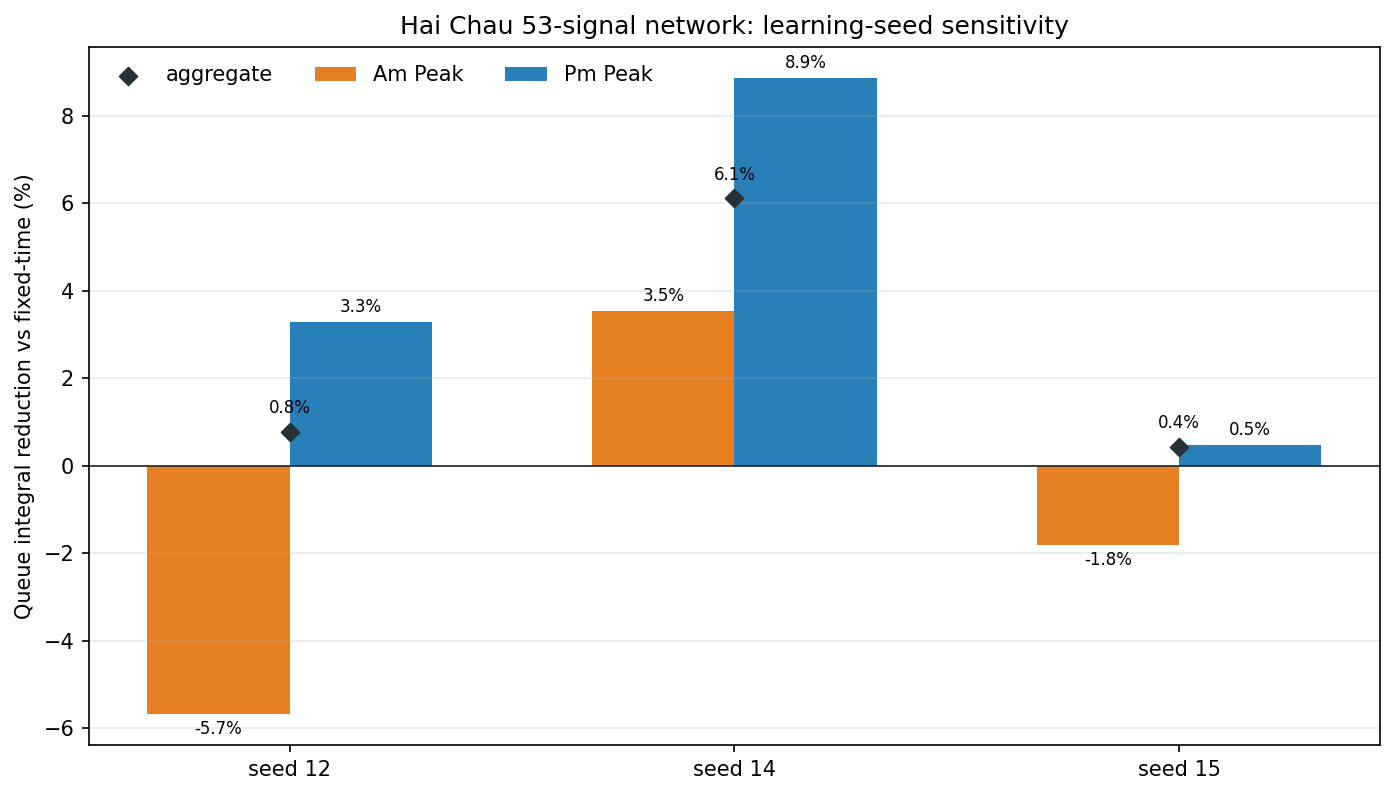
\includegraphics[width=0.82\textwidth]{../results/haichau_network_v2/final15-seed-sensitivity.png}
\caption{Learning-seed sensitivity on the complete fifteen-case Hai Chau matrix. Diamonds show aggregate reduction; bars separate AM and PM peak effects.}
\label{fig:seed-sensitivity}
\end{figure}

For context, the same fifteen cases were evaluated with two non-learning
baselines. Max-Pressure accumulated 6,347.00 vehicle-hours and hysteretic
Max-Pressure 6,739.13, compared with 8,339.43 for fixed-time. Their aggregate
reductions were therefore 23.89\% and 19.19\%, while schedule-residual DDQN
reduced the metric by 6.12\%. Max-Pressure is the strongest controller in this
synthetic matrix; the thesis consequently claims improvement over fixed-time,
not universal superiority over every baseline. The complete matrix is stored
in \path{results/haichau_network_v2/final15-controller-matrix-summary.json}.

The same fifteen matched seed-14 cases provide secondary operational outcomes.
Residual DDQN increases mean completion from $66.92\%$ to $67.98\%$ (+1.06
percentage points) and insertion from $97.15\%$ to $97.97\%$ (+0.82 points).
The mean maximum queue at a signal falls from 141.87 to 124.93 vehicles.
Completed-trip travel time rises slightly from 737.81 to 743.26 seconds, and
spillback lane-seconds rise from 1,432.33 to 1,497.53 overall. The AM spillback
increase (1,144.8 to 1,461.0 lane-seconds) and PM decrease (2,751.4 to 2,630.8)
show why queue reduction is not interpreted as universal travel-time or
spillback improvement. These descriptive outcomes are generated from
\path{results/haichau_network_v2/final15-seed14-secondary-summary.json} and do
not replace seed-level inference.

For the defense, a self-contained replay bundle at
\path{results/haichau_network_v2/demo-visual} shows a matched PM-peak visual
comparison without requiring CityFlow or network access. It is illustrative;
the thesis conclusions use the complete evaluation artifacts.

\section{Answer to the research question}
RQ1 is answered by a traceable reconstruction using published partial counts and declared assumptions; behavioral and full-junction calibration remain unsupported. RQ2 finds substantial normal-demand degradation, unresolved AM difference, and a PM benefit within the corrected SUMO model. RQ3 finds that schedule-residual DDQN can execute across 53 synthetic signal agents and improve on fixed-time in the selected bounded matrix, while both pressure baselines obtain larger aggregate reductions. The five-seed post hoc gate is exploratory and has case-level regressions. RQ4 is answered negatively for strict confirmation: the release is incomplete, two residual seeds failed validation selection, and the gate lacks a new untouched evaluation set. These outcomes support a reproducible simulation case study with explicit failure analysis, not a deployment recommendation.

\chapter{Discussion}\label{ch:discussion}

\section{Why performance changes with demand}
At low demand, the published plan clears the small queues efficiently and predictably. A learned policy has little congestion to recover but can still pay clearance costs or starve a minor movement. At high demand, queues persist across cycles, so responding to imbalance can recover more time than switching costs consume. The PM profile and scaled stress tests expose this advantage. Seed variability shows that architecture alone does not guarantee a good policy.

\section{Implications for deployment}
The single-junction simulation motivates a candidate demand or queue threshold for deciding when to use DDQN and when to retain the published plan. Such a rule is a hypothesis for later field validation, not a deployment recommendation from the present evidence. Any operational study would have to enforce minimum-green and clearance rules outside the neural network, monitor out-of-distribution state ranges, log pending demand as well as visible queues, and begin with shadow-mode evaluation using live detectors and independent traffic-engineering review.

\section{Threats to validity}
\textbf{Construct validity.} The primary metric measures queue accumulation, not emissions, pedestrian delay, equity, or field travel time. Four camera lines do not observe the entire anchor junction, and digitization introduces reading error. The stated $\pm15/\pm30$ values are project reading tolerances, not detector accuracy or 95\% measurement intervals; that uncertainty has not been propagated through training and evaluation. At network scale, synthetic departure intensity inherits only the relative temporal shape of those lines; it is not a measurement of OD demand across Hai Chau. Completed-vehicle travel time is subject to survivorship bias when completion differs, so it is always accompanied by pending and unfinished counts.

\textbf{Internal validity.} The isolated network removes neighboring confounding but also removes spillback. Driver parameters are engineering assumptions. A single headway change removed a reproduced collision, but no trajectory data support full car-following calibration. The change was prompted by a held-out case, so the reused test set is development-informed. The network PM-only gate was also chosen after test inspection. Fresh execution does not remove either source of adaptation bias. In CityFlow, inferred green-phase roles, synthetic fixed-time plans, route sampling, vehicle templates, downstream-capacity proxies, and the chosen reward weights can change controller rankings. Hashes make those choices reproducible; they do not validate them against the street. The network fixed-time baseline is a validation-tuned uncoordinated plan without offsets. Coordinated green-wave timing, as studied for several Da Nang arterials~\cite{tran2007greenwave}, would be a stronger fixed-time baseline and was not tested. The isolated junction has no neighbor to coordinate with, so this limitation applies to the network tier only.

\textbf{External validity.} Camera observations cover one date, while the separate movement table is based on 2022 data. Departure seeds vary routes and timing inside the generator, not independent survey days. OpenStreetMap topology does not confirm the current field inventory or timing of all 53 signals. Neither the single-junction findings nor a passing synthetic-network result generalizes automatically to another hour, weather condition, incident, district, or all of Da Nang.

\textbf{Statistical conclusion validity.} Five training seeds give only moderate precision. Bootstrap intervals expose algorithmic uncertainty but cannot repair limited independent traffic data. The single-junction architecture ablation uses one seed and combines two changes, so it supports selection within that experiment rather than a general claim about dueling or $n$-step learning. The network analysis avoids treating agents, time steps, or crossed simulator runs as independent, but five seed-level units still limit power; passing a predeclared gate supports only the frozen task family.

\textbf{Network-extension statistical conclusion validity.} The five-seed gate interval is conditional on the retained cases, diagnostic checkpoint choices, and post hoc gate; it does not establish confirmatory coverage after selection. Normal/AM ties are structural fallback behavior rather than evidence of learned non-inferiority. The original proposed either-peak acceptance rule uses pointwise intervals without multiplicity correction. Neither that rule nor bootstrap intervals compensate for missing independent field days.

\section{What was rejected}
The legacy project described a 53-intersection Hai Chau network and 50,500 real trips. The repository did not contain evidence sufficient to support the real-trip claim, so those historical rows remain immutable legacy evidence. The new extension uses a versioned namespace, a 53-signal OpenStreetMap-derived topology, matched controller runs, and synthetic network demand constrained by Da Nang evidence. The bounded result in the Results chapter is evidence from the completed cases; it cannot replace the isolated-junction empirical evidence or be presented as the strict five-seed confirmatory release.

\section{Hai Chau network result status}
The strict frozen 53-signal release artifacts are absent. The completed bounded evidence is reported in the Results chapter. The strict verifier reports failure; this status is preserved rather than replaced by a presentation-readiness flag. The source ledger and audit report in Appendix~\ref{app:evidence} distinguish retained summaries from absent release artifacts.

\chapter{Reproducibility and Defense Demonstration}\label{ch:reproducibility}

\section{Artifact structure}
The repository stores source observations under \texttt{datasets/danang\_published}, single-junction network and calibration evidence under \texttt{results/research\_pilot}, and its frozen protocol under \texttt{results/danang\_protocol\_v1}. The district-scale dataset and case manifest use \texttt{datasets/haichau\_network\_v2} and \texttt{results/haichau\_network\_v2}; generated results remain in that namespace. Reported aggregates can be traced to JSON evaluation records. The manuscript contains rounded table values, which are independently reconciled by the evidence audit. The source PDF, source-page locators, CSVs, selection snapshots, and checksums are indexed in \path{docs/research/thesis-evidence-ledger.md}.

\section{Presentation-safe demo}
The supported demonstration is the self-contained recorded PM replay at \path{results/haichau_network_v2/demo-visual}. It illustrates matched controller behavior at selected times. A visible queue difference is a snapshot, not a causal count of additional vehicles discharged, and it cannot replace a complete matched evaluation. Vehicle glyphs, road geometry, and smooth playback do not validate field traffic. The demonstration is labelled synthetic and exploratory; neither the retired bounded viewer nor the defense slides are prerequisites for reading the retained quantitative results.

\section{Reproduction sequence}
Scenario preparation, training, held-out evaluation, statistical summarization, thesis compilation, and demo export are separate stages. Appendix~\ref{app:repro} lists the commands; manifests retain available checksums and runtime metadata.

\chapter{Conclusion and Future Work}\label{ch:conclusion}

This thesis separates two questions that available public data cannot answer with one model. The empirical anchor reconstructs and evaluates an adaptive controller at a published Da Nang signal under explicit evidence limits. In that simulation, \ddqn{} reduced queue accumulation at the PM peak and high synthetic demand, did not resolve a difference at the observed AM profile, and performed worse in normal traffic. The result motivates a demand-gated research hypothesis with fixed-time fallback; it does not establish readiness for field operation.

The district-scale tier contributes an executable 53-signal CityFlow task, a schedule-residual Double DQN, and matched synthetic comparisons. In the bounded seed-14 matrix, queue integral is 6.12\% below tuned fixed-time, while Max-Pressure achieves 23.89\%. A post hoc PM-only gate yields a mean pooled-case reduction of 3.48\% across five diagnostic learning runs. Two of those runs failed the original validation selector. The result is exploratory, and independent confirmation plus a complete release package remain outstanding. The study's value includes documenting these limits and negative comparisons rather than asserting universal RL superiority.

Across both tiers, a held-out collision forced a headway correction and complete rerun, seed-level uncertainty replaced a single headline percentage with regime-specific conclusions, and pending-demand accounting prevented boundary blocking from looking efficient. These protocol practices are transferable to other traffic RL studies.

The public-camera demonstration (Section~\ref{sec:camera}) suggests a practical route to such data: the next steps are a manual count to measure detection and identity accuracy, better far-field motorcycle detection, and several days of video before any count is used for demand calibration. A coordinated green-wave fixed-time plan should also be added as a network baseline. Future work should collect multi-day, full-movement counts, queues, headways, travel times, pedestrian demand, signal logs, and district OD or detector records. Those data would permit behavioral calibration, independent-day testing, and replacement of synthetic network timings and routes with measured inputs. A field-calibrated spatial study can begin with the nearby Nui Thanh and Thang Long signals before expanding through Hai Chau, so spillback and coordination claims grow with the evidence base. Algorithmically, learned graph attention, uncertainty-aware policy ensembles, demand gating, constrained switching, and offline pretraining from signal logs deserve evaluation. Field deployment should begin in shadow mode and advance only after independent safety and traffic-engineering review.

\appendix
\chapter{Reproduction Commands}\label{app:repro}
Run these commands from the repository root. The audit checks retained evidence without training. The strict verifier is expected to return nonzero until the missing release is completed.
\begin{lstlisting}[basicstyle=\ttfamily\small,breaklines=true]
python3 scripts/audit_thesis_evidence.py
PYTHONPATH=src python3 scripts/verify_haichau_foundation.py
PYTHONPATH=src python3 scripts/verify_haichau_thesis.py --no-write
python3 scripts/run_danang_baseline_mc.py --parity
python3 scripts/run_danang_baseline_mc.py -n 1000 -j 10
python3 scripts/plot_danang_baseline_mc.py
python3 scripts/count_camera_vehicles.py --video <local video> --config configs/camera/caurong_20260711.json --model <yolov8x-visdrone weights> --out results/camera_counts/caurong_20260711_1716 --start-clock 17:15:59
python3 scripts/analyze_camera_routes.py results/camera_counts/caurong_20260711_1716 --only car
tectonic paper/thesis_danang.tex
cd results/haichau_network_v2/demo-visual
python3 launch_demo.py --no-browser --port 8766
\end{lstlisting}
The first command verifies the source PDF checksum, transcribed table, camera totals, retained evaluation means, seed-level gate calculations, and selection snapshots. Its success is not a strict release acceptance. The camera commands need the locally downloaded video and detector weights, which are not distributed in Git; \path{results/camera_counts/README.md} records their sources. The SUMO scripts \path{scripts/prepare_danang_protocol.py}, \path{scripts/train_danang_sumo.py}, and \path{scripts/evaluate_danang_protocol.py} define the original generation/training/evaluation workflow. Reproduction of CityFlow raw episodes additionally requires the digest-pinned runtime and local checkpoint bytes described by their original contracts; the audit does not claim a fresh clone can regenerate all episodes unaided. New confirmation must use a newly frozen protocol and uninspected demand realizations, with its status reported separately.

\chapter{Parameter Ledger}
\section{Empirical single-junction SUMO experiment}
\begin{longtable}{>{\raggedright\arraybackslash}p{4cm}>{\raggedright\arraybackslash}p{3cm}>{\raggedright\arraybackslash}p{6cm}}
\caption{Final parameters for the empirical-anchor SUMO experiment.}\\
\toprule Parameter & Value & Rationale \\
\midrule\endfirsthead
\toprule Parameter & Value & Rationale \\
\midrule\endhead
Simulation horizon & 3,600 s & One-hour camera-supported scenario \\
Decision interval & 10 s & Responsive control with bounded action rate \\
Minimum green & 20 s & Avoid rapid oscillation \\
Yellow/clearance & 7 s & Published site plan \\
Motorcycle headway & 1.2 s & Held-out collision regression \\
Training episodes & 30 & Fixed compute budget for every seed \\
Training seeds & 11--15 & Independent learned policies \\
Discount factor & 0.99 & Long-horizon queue objective \\
Replay capacity & 50,000 & Covers the training decision stream \\
Batch size & 64 & Stable mini-batch updates \\
Learning rate & 0.0003 & Shared across ablation and final model \\
Target sync & 200 updates & Stabilizes temporal-difference targets \\
$n$-step return & 3 & Selected with dueling architecture ablation \\
Hidden width & 64 & Compact deployable network \\
Validation frequency & 5 episodes & Six full-hour selection checkpoints \\
Bootstrap replicates & 20,000 & Stable interval computation \\
\bottomrule
\end{longtable}

\section{District-scale CityFlow experiment}
\begin{longtable}{>{\raggedright\arraybackslash}p{3.5cm}>{\raggedright\arraybackslash}p{3.0cm}>{\raggedright\arraybackslash}p{6.5cm}}
\caption{Parameters of the retained residual-controller runs; later candidate configurations do not redefine these results.}\\
\toprule Parameter & Value & Evidence/meaning \\
\midrule\endfirsthead
\toprule Parameter & Value & Evidence/meaning \\
\midrule\endhead
Controlled signals & 53 & OSM-derived synthetic task \\
Case split & 9/6/15 & Train/validation/test \\
Episode horizon & 3,600 s & Independent one-hour episodes \\
Route streams/case & 500 & Sampled from 1,290 partitioned families \\
Motorcycle share & 0.90 & Synthetic assumption \\
Reference green & 25 s & Validation-tuned fixed-time \\
Macro duration/shift & 300 / $\pm10$ s & Compiled schedule modifications \\
Minimum green/max red & 20/180 s & Configured constraints; phase contract also applies \\
Action interval & 10 s & Simulator control interval \\
Training episodes & 12 & Retained resolved configuration \\
Validation checkpoints & 4/8/12 & Full validation evaluations \\
Model input/hidden & 27 / 64,64 & Shared scalar-scoring Double DQN \\
Dueling heads & None & Distinct from SUMO dueling agent \\
Replay capacity/start & 20,000/53 & Residual optimizer configuration \\
Batch size & 128 & Residual optimizer configuration \\
Learning rate & 0.0003 & Residual optimizer configuration \\
Updates per macro & 8 & Residual optimizer configuration \\
Target sync & 64 updates & Residual optimizer configuration \\
Return/discount & SMDP / 0.99 & Discount per 300-second macro \\
Reward & Negative queue integral & Network plus pending; critic divisor 100,000 \\
Learning seeds & 12--16 & Seeds 13 and 16 rejected by selector \\
Gate bootstrap & 10,000 & Resamples five seed effects; seed 20260913 \\
\bottomrule
\end{longtable}

\chapter{Claim-to-Evidence Matrix}\label{app:evidence}
The source-of-truth ledger is \path{docs/research/thesis-evidence-ledger.md}, with machine-readable checksums and recalculated values in \path{docs/research/thesis-evidence-audit.json}. The source PDF is retained under \path{datasets/danang_published/sources/}. Source-page numbers below refer to the article's printed pages (24 pages total).

Bibliographic identity checks are recorded in \path{docs/research/bibliography-metadata-audit.json}: 51 DOI/title matches and 19 other primary-source identities, re-screened on 11 October 2026 against Crossref, arXiv, and publisher pages. The original Webster (1958) report was not obtained; its identity and classical formulation are corroborated indirectly by FHWA. Metadata matching does not verify every full-text claim. The SURTRAC citation was corrected against CMU's conference record. The experimental data sources receive the more specific page/table/figure audit below.

\begin{longtable}{>{\raggedright\arraybackslash}p{4.0cm}>{\raggedright\arraybackslash}p{9.0cm}}
\toprule Claim & Evidence and permitted interpretation \\
\midrule\endfirsthead
\toprule Claim & Evidence and permitted interpretation \\
\midrule\endhead
Historical 103-second plan & Phan et al., p.~7 and Fig.~4, p.~8: green 32/28/22 s and three 7 s yellows. Not a current field timing survey. \\
12 movements, 6,171 PCU/h & Table~1, p.~8; attribution to 2022 data on p.~7. CSV transcribes every movement. Original authority dataset was not obtained. \\
48 camera rows & Collection date/window p.~16; Fig.~12 p.~17; Figs.~17--18 p.~20. Twelve plot labels for four movements; approximate published counts. \\
PCU conversion & p.~19: motorcycle 0.3, car 1, bus 2, truck 2.5. Derived PCU is not an additional observation. \\
Raw data restriction & Data Availability Statement, p.~23. Public article access does not release raw camera or authority data. \\
SUMO comparison & \path{results/danang_protocol_v1/evaluation/}: 120 one-hour records, including 75 learned and 45 baseline runs. Summary under \path{results/danang_protocol_v1/summary/}. \\
Baseline Monte-Carlo & \path{results/danang_baseline_mc/runs.jsonl} and \path{summary.json}: 9,000 paired runs, 1,000 realizations per regime, seeds disjoint from the protocol; realizations of one observed profile, not independent days. \\
Public-camera YOLO counts & \path{results/camera_counts/caurong_20260711_1716/} (\path{meta.json}, \path{entries_exits.csv}, \path{only_car/}) and \path{results/camera_counts/realtime_check_m1280_s4/timing.json}. Feasibility only: no hand count, far-field motorcycles under-counted, no simulator input. \\
Green-wave context & Tran and Phan (2007), abstract only (Tap chi Cau Duong Viet Nam, no.~10/2007, pp.~23--28). Local framing; no timing value or count is taken from it. \\
Demand sensitivity & \path{results/danang_protocol_v1/sensitivity/}: 120 records, synthetic scales around the camera-derived AM profile; 1.00-scale outcomes repeat the primary AM conditions. \\
53-signal topology & \path{datasets/haichau_network_v2/provenance.json} and \path{results/haichau_network_v2/experiment-manifest.json}; synthetic demand, unknown original retrieval date. \\
Four-controller comparison & \path{results/haichau_network_v2/final15-controller-matrix-summary.json}; one selected residual seed, not five-seed confirmation. \\
Five-seed post hoc gate & \path{results/haichau_network_v2/final15-regime-gated-direct-multi-seed-summary.json}; conditional exploratory effects. \\
Rejected seeds 13/16 & Byte-identical selector snapshots in \path{docs/research/evidence-snapshot-2026-09-23/}. A diagnostic replay does not overturn rejection. \\
Strict release status & Fresh \texttt{verify\_haichau\_thesis.py --no-write} report retained in the evidence audit: incomplete. Absent final artifacts are not cited as completed evidence. \\
\bottomrule
\end{longtable}

\bibliographystyle{plainnat}
\bibliography{references_verified}

\end{document}
